% Options for packages loaded elsewhere
\PassOptionsToPackage{unicode}{hyperref}
\PassOptionsToPackage{hyphens}{url}
\documentclass[
]{article}
\usepackage{xcolor}
\usepackage[margin=1in]{geometry}
\usepackage{amsmath,amssymb}
\setcounter{secnumdepth}{-\maxdimen} % remove section numbering
\usepackage{iftex}
\ifPDFTeX
  \usepackage[T1]{fontenc}
  \usepackage[utf8]{inputenc}
  \usepackage{textcomp} % provide euro and other symbols
\else % if luatex or xetex
  \usepackage{unicode-math} % this also loads fontspec
  \defaultfontfeatures{Scale=MatchLowercase}
  \defaultfontfeatures[\rmfamily]{Ligatures=TeX,Scale=1}
\fi
\usepackage{lmodern}
\ifPDFTeX\else
  % xetex/luatex font selection
\fi
% Use upquote if available, for straight quotes in verbatim environments
\IfFileExists{upquote.sty}{\usepackage{upquote}}{}
\IfFileExists{microtype.sty}{% use microtype if available
  \usepackage[]{microtype}
  \UseMicrotypeSet[protrusion]{basicmath} % disable protrusion for tt fonts
}{}
\makeatletter
\@ifundefined{KOMAClassName}{% if non-KOMA class
  \IfFileExists{parskip.sty}{%
    \usepackage{parskip}
  }{% else
    \setlength{\parindent}{0pt}
    \setlength{\parskip}{6pt plus 2pt minus 1pt}}
}{% if KOMA class
  \KOMAoptions{parskip=half}}
\makeatother
\usepackage{color}
\usepackage{fancyvrb}
\newcommand{\VerbBar}{|}
\newcommand{\VERB}{\Verb[commandchars=\\\{\}]}
\DefineVerbatimEnvironment{Highlighting}{Verbatim}{commandchars=\\\{\}}
% Add ',fontsize=\small' for more characters per line
\usepackage{framed}
\definecolor{shadecolor}{RGB}{248,248,248}
\newenvironment{Shaded}{\begin{snugshade}}{\end{snugshade}}
\newcommand{\AlertTok}[1]{\textcolor[rgb]{0.94,0.16,0.16}{#1}}
\newcommand{\AnnotationTok}[1]{\textcolor[rgb]{0.56,0.35,0.01}{\textbf{\textit{#1}}}}
\newcommand{\AttributeTok}[1]{\textcolor[rgb]{0.13,0.29,0.53}{#1}}
\newcommand{\BaseNTok}[1]{\textcolor[rgb]{0.00,0.00,0.81}{#1}}
\newcommand{\BuiltInTok}[1]{#1}
\newcommand{\CharTok}[1]{\textcolor[rgb]{0.31,0.60,0.02}{#1}}
\newcommand{\CommentTok}[1]{\textcolor[rgb]{0.56,0.35,0.01}{\textit{#1}}}
\newcommand{\CommentVarTok}[1]{\textcolor[rgb]{0.56,0.35,0.01}{\textbf{\textit{#1}}}}
\newcommand{\ConstantTok}[1]{\textcolor[rgb]{0.56,0.35,0.01}{#1}}
\newcommand{\ControlFlowTok}[1]{\textcolor[rgb]{0.13,0.29,0.53}{\textbf{#1}}}
\newcommand{\DataTypeTok}[1]{\textcolor[rgb]{0.13,0.29,0.53}{#1}}
\newcommand{\DecValTok}[1]{\textcolor[rgb]{0.00,0.00,0.81}{#1}}
\newcommand{\DocumentationTok}[1]{\textcolor[rgb]{0.56,0.35,0.01}{\textbf{\textit{#1}}}}
\newcommand{\ErrorTok}[1]{\textcolor[rgb]{0.64,0.00,0.00}{\textbf{#1}}}
\newcommand{\ExtensionTok}[1]{#1}
\newcommand{\FloatTok}[1]{\textcolor[rgb]{0.00,0.00,0.81}{#1}}
\newcommand{\FunctionTok}[1]{\textcolor[rgb]{0.13,0.29,0.53}{\textbf{#1}}}
\newcommand{\ImportTok}[1]{#1}
\newcommand{\InformationTok}[1]{\textcolor[rgb]{0.56,0.35,0.01}{\textbf{\textit{#1}}}}
\newcommand{\KeywordTok}[1]{\textcolor[rgb]{0.13,0.29,0.53}{\textbf{#1}}}
\newcommand{\NormalTok}[1]{#1}
\newcommand{\OperatorTok}[1]{\textcolor[rgb]{0.81,0.36,0.00}{\textbf{#1}}}
\newcommand{\OtherTok}[1]{\textcolor[rgb]{0.56,0.35,0.01}{#1}}
\newcommand{\PreprocessorTok}[1]{\textcolor[rgb]{0.56,0.35,0.01}{\textit{#1}}}
\newcommand{\RegionMarkerTok}[1]{#1}
\newcommand{\SpecialCharTok}[1]{\textcolor[rgb]{0.81,0.36,0.00}{\textbf{#1}}}
\newcommand{\SpecialStringTok}[1]{\textcolor[rgb]{0.31,0.60,0.02}{#1}}
\newcommand{\StringTok}[1]{\textcolor[rgb]{0.31,0.60,0.02}{#1}}
\newcommand{\VariableTok}[1]{\textcolor[rgb]{0.00,0.00,0.00}{#1}}
\newcommand{\VerbatimStringTok}[1]{\textcolor[rgb]{0.31,0.60,0.02}{#1}}
\newcommand{\WarningTok}[1]{\textcolor[rgb]{0.56,0.35,0.01}{\textbf{\textit{#1}}}}
\usepackage{longtable,booktabs,array}
\newcounter{none} % for unnumbered tables
\usepackage{calc} % for calculating minipage widths
% Correct order of tables after \paragraph or \subparagraph
\usepackage{etoolbox}
\makeatletter
\patchcmd\longtable{\par}{\if@noskipsec\mbox{}\fi\par}{}{}
\makeatother
% Allow footnotes in longtable head/foot
\IfFileExists{footnotehyper.sty}{\usepackage{footnotehyper}}{\usepackage{footnote}}
\makesavenoteenv{longtable}
\usepackage{graphicx}
\makeatletter
\newsavebox\pandoc@box
\newcommand*\pandocbounded[1]{% scales image to fit in text height/width
  \sbox\pandoc@box{#1}%
  \Gscale@div\@tempa{\textheight}{\dimexpr\ht\pandoc@box+\dp\pandoc@box\relax}%
  \Gscale@div\@tempb{\linewidth}{\wd\pandoc@box}%
  \ifdim\@tempb\p@<\@tempa\p@\let\@tempa\@tempb\fi% select the smaller of both
  \ifdim\@tempa\p@<\p@\scalebox{\@tempa}{\usebox\pandoc@box}%
  \else\usebox{\pandoc@box}%
  \fi%
}
% Set default figure placement to htbp
\def\fps@figure{htbp}
\makeatother
\setlength{\emergencystretch}{3em} % prevent overfull lines
\providecommand{\tightlist}{%
  \setlength{\itemsep}{0pt}\setlength{\parskip}{0pt}}
\usepackage{bookmark}
\IfFileExists{xurl.sty}{\usepackage{xurl}}{} % add URL line breaks if available
\urlstyle{same}
\hypersetup{
  pdftitle={Assignment 3},
  pdfauthor={Will, Taylor, Nikhil, Abe},
  hidelinks,
  pdfcreator={LaTeX via pandoc}}

\title{Assignment 3}
\author{Will, Taylor, Nikhil, Abe}
\date{2025-11-12}

\begin{document}
\maketitle

\section{Package Installation}\label{package-installation}

\begin{Shaded}
\begin{Highlighting}[]
\FunctionTok{options}\NormalTok{(}\AttributeTok{repos =} \FunctionTok{c}\NormalTok{(}\AttributeTok{CRAN =} \StringTok{"https://cloud.r{-}project.org"}\NormalTok{))}
\FunctionTok{suppressPackageStartupMessages}\NormalTok{(}\FunctionTok{library}\NormalTok{(readr))}
\FunctionTok{suppressPackageStartupMessages}\NormalTok{(}\FunctionTok{library}\NormalTok{(dplyr))}
\FunctionTok{suppressPackageStartupMessages}\NormalTok{(}\FunctionTok{library}\NormalTok{(tibble))}
\NormalTok{cran\_pkgs }\OtherTok{\textless{}{-}} \FunctionTok{c}\NormalTok{(}
  \StringTok{"tidyr"}\NormalTok{,}\StringTok{"purrr"}\NormalTok{,}\StringTok{"janitor"}\NormalTok{,}\StringTok{"glue"}\NormalTok{,}\StringTok{"mclust"}\NormalTok{,}
  \StringTok{"matrixStats"}\NormalTok{,}\StringTok{"cluster"}\NormalTok{,}\StringTok{"forcats"}\NormalTok{,}\StringTok{"RColorBrewer"}\NormalTok{,}\StringTok{"scales"}\NormalTok{,}
  \StringTok{"magick"}\NormalTok{,}\StringTok{"Cairo"}\NormalTok{,}\StringTok{"factoextra"}\NormalTok{,}\StringTok{"pheatmap"}
\NormalTok{)}
\NormalTok{to\_install }\OtherTok{\textless{}{-}} \FunctionTok{setdiff}\NormalTok{(cran\_pkgs, }\FunctionTok{rownames}\NormalTok{(}\FunctionTok{installed.packages}\NormalTok{()))}
\ControlFlowTok{if}\NormalTok{ (}\FunctionTok{length}\NormalTok{(to\_install)) }\FunctionTok{install.packages}\NormalTok{(to\_install)}

\ControlFlowTok{if}\NormalTok{ (}\SpecialCharTok{!}\FunctionTok{requireNamespace}\NormalTok{(}\StringTok{"BiocManager"}\NormalTok{, }\AttributeTok{quietly =} \ConstantTok{TRUE}\NormalTok{)) }\FunctionTok{install.packages}\NormalTok{(}\StringTok{"BiocManager"}\NormalTok{)}
\NormalTok{BiocManager}\SpecialCharTok{::}\FunctionTok{install}\NormalTok{(}\FunctionTok{c}\NormalTok{(}\StringTok{"ComplexHeatmap"}\NormalTok{,}\StringTok{"circlize"}\NormalTok{), }\AttributeTok{update =} \ConstantTok{FALSE}\NormalTok{, }\AttributeTok{ask =} \ConstantTok{FALSE}\NormalTok{)}
\end{Highlighting}
\end{Shaded}

\begin{verbatim}
## Warning: package(s) not installed when version(s) same as or greater than current; use
##   `force = TRUE` to re-install: 'ComplexHeatmap' 'circlize'
\end{verbatim}

\begin{Shaded}
\begin{Highlighting}[]
\FunctionTok{library}\NormalTok{(ggplot2)}
\end{Highlighting}
\end{Shaded}

\section{Section 1}\label{section-1}

\begin{Shaded}
\begin{Highlighting}[]
\NormalTok{data\_dir }\OtherTok{\textless{}{-}} \FunctionTok{file.path}\NormalTok{(}\StringTok{"data"}\NormalTok{, }\StringTok{"SRP192714"}\NormalTok{)}
\NormalTok{counts\_path }\OtherTok{\textless{}{-}} \FunctionTok{file.path}\NormalTok{(data\_dir, }\StringTok{"SRP192714.tsv"}\NormalTok{)}
\NormalTok{metadata\_path }\OtherTok{\textless{}{-}} \FunctionTok{file.path}\NormalTok{(data\_dir, }\StringTok{"metadata\_SRP192714\_merged.tsv"}\NormalTok{)}

\FunctionTok{stopifnot}\NormalTok{(}\FunctionTok{file.exists}\NormalTok{(counts\_path))}

\ControlFlowTok{if}\NormalTok{ (}\SpecialCharTok{!}\FunctionTok{file.exists}\NormalTok{(metadata\_path)) \{}
    \FunctionTok{message}\NormalTok{(}\StringTok{"Rebuilding merged metadata from Assignment2 inputs..."}\NormalTok{)}
\NormalTok{    refinebio\_path }\OtherTok{\textless{}{-}} \FunctionTok{file.path}\NormalTok{(data\_dir, }\StringTok{"metadata\_SRP192714.tsv"}\NormalTok{)}
\NormalTok{    geo\_path }\OtherTok{\textless{}{-}} \FunctionTok{file.path}\NormalTok{(}\StringTok{"data"}\NormalTok{, }\StringTok{"GSE129882\_PhenoData.transcript.csv"}\NormalTok{)}
    \FunctionTok{stopifnot}\NormalTok{(}\FunctionTok{file.exists}\NormalTok{(refinebio\_path), }\FunctionTok{file.exists}\NormalTok{(geo\_path))}

\NormalTok{    refinebio\_meta }\OtherTok{\textless{}{-}}\NormalTok{ readr}\SpecialCharTok{::}\FunctionTok{read\_tsv}\NormalTok{(refinebio\_path, }\AttributeTok{show\_col\_types =} \ConstantTok{FALSE}\NormalTok{)}
\NormalTok{    geo\_meta }\OtherTok{\textless{}{-}}\NormalTok{ readr}\SpecialCharTok{::}\FunctionTok{read\_csv}\NormalTok{(geo\_path, }\AttributeTok{show\_col\_types =} \ConstantTok{FALSE}\NormalTok{)}

    \ControlFlowTok{if}\NormalTok{ (}\StringTok{"Sample"} \SpecialCharTok{\%in\%} \FunctionTok{names}\NormalTok{(geo\_meta) }\SpecialCharTok{\&\&} \StringTok{"refinebio\_title"} \SpecialCharTok{\%in\%} \FunctionTok{names}\NormalTok{(refinebio\_meta)) \{}
\NormalTok{        merged\_meta }\OtherTok{\textless{}{-}}\NormalTok{ dplyr}\SpecialCharTok{::}\FunctionTok{left\_join}\NormalTok{(}
\NormalTok{            refinebio\_meta,}
\NormalTok{            geo\_meta,}
            \AttributeTok{by =} \FunctionTok{c}\NormalTok{(}\StringTok{"refinebio\_title"} \OtherTok{=} \StringTok{"Sample"}\NormalTok{)}
\NormalTok{        )}
\NormalTok{    \} }\ControlFlowTok{else}\NormalTok{ \{}
\NormalTok{        merged\_meta }\OtherTok{\textless{}{-}}\NormalTok{ refinebio\_meta}
\NormalTok{    \}}

\NormalTok{    readr}\SpecialCharTok{::}\FunctionTok{write\_tsv}\NormalTok{(merged\_meta, metadata\_path)}
\NormalTok{\}}

\NormalTok{counts\_df }\OtherTok{\textless{}{-}}\NormalTok{ readr}\SpecialCharTok{::}\FunctionTok{read\_tsv}\NormalTok{(counts\_path, }\AttributeTok{show\_col\_types =} \ConstantTok{FALSE}\NormalTok{)}
\FunctionTok{stopifnot}\NormalTok{(}\StringTok{"Gene"} \SpecialCharTok{\%in\%} \FunctionTok{names}\NormalTok{(counts\_df))}

\NormalTok{expression\_mat }\OtherTok{\textless{}{-}}\NormalTok{ counts\_df }\SpecialCharTok{\%\textgreater{}\%}
    \FunctionTok{column\_to\_rownames}\NormalTok{(}\StringTok{"Gene"}\NormalTok{) }\SpecialCharTok{\%\textgreater{}\%}
    \FunctionTok{as.matrix}\NormalTok{()}
\FunctionTok{mode}\NormalTok{(expression\_mat) }\OtherTok{\textless{}{-}} \StringTok{"numeric"}

\NormalTok{metadata }\OtherTok{\textless{}{-}}\NormalTok{ readr}\SpecialCharTok{::}\FunctionTok{read\_tsv}\NormalTok{(metadata\_path, }\AttributeTok{show\_col\_types =} \ConstantTok{FALSE}\NormalTok{)}
\FunctionTok{stopifnot}\NormalTok{(}\FunctionTok{all}\NormalTok{(}\FunctionTok{c}\NormalTok{(}\StringTok{"refinebio\_accession\_code"}\NormalTok{, }\StringTok{"Exposure"}\NormalTok{) }\SpecialCharTok{\%in\%} \FunctionTok{names}\NormalTok{(metadata)))}

\NormalTok{common\_samples }\OtherTok{\textless{}{-}} \FunctionTok{intersect}\NormalTok{(}\FunctionTok{colnames}\NormalTok{(expression\_mat), metadata}\SpecialCharTok{$}\NormalTok{refinebio\_accession\_code)}
\FunctionTok{stopifnot}\NormalTok{(}\FunctionTok{length}\NormalTok{(common\_samples) }\SpecialCharTok{\textgreater{}} \DecValTok{0}\NormalTok{)}

\NormalTok{common\_samples }\OtherTok{\textless{}{-}} \FunctionTok{sort}\NormalTok{(common\_samples)}
\NormalTok{expression\_mat }\OtherTok{\textless{}{-}}\NormalTok{ expression\_mat[, common\_samples, drop }\OtherTok{=} \ConstantTok{FALSE}\NormalTok{]}

\NormalTok{metadata }\OtherTok{\textless{}{-}}\NormalTok{ metadata }\SpecialCharTok{\%\textgreater{}\%}
    \FunctionTok{filter}\NormalTok{(refinebio\_accession\_code }\SpecialCharTok{\%in\%}\NormalTok{ common\_samples) }\SpecialCharTok{\%\textgreater{}\%}
    \FunctionTok{mutate}\NormalTok{(}\AttributeTok{refinebio\_accession\_code =} \FunctionTok{factor}\NormalTok{(refinebio\_accession\_code, }\AttributeTok{levels =}\NormalTok{ common\_samples)) }\SpecialCharTok{\%\textgreater{}\%}
    \FunctionTok{arrange}\NormalTok{(refinebio\_accession\_code)}

\NormalTok{metadata}\SpecialCharTok{$}\NormalTok{Exposure }\OtherTok{\textless{}{-}} \FunctionTok{droplevels}\NormalTok{(}\FunctionTok{factor}\NormalTok{(metadata}\SpecialCharTok{$}\NormalTok{Exposure))}

\FunctionTok{stopifnot}\NormalTok{(}\FunctionTok{identical}\NormalTok{(}\FunctionTok{colnames}\NormalTok{(expression\_mat), }\FunctionTok{as.character}\NormalTok{(metadata}\SpecialCharTok{$}\NormalTok{refinebio\_accession\_code)))}

\FunctionTok{cat}\NormalTok{(}\StringTok{"Genes loaded:"}\NormalTok{, }\FunctionTok{nrow}\NormalTok{(expression\_mat), }\StringTok{"}\SpecialCharTok{\textbackslash{}n}\StringTok{"}\NormalTok{)}
\end{Highlighting}
\end{Shaded}

\begin{verbatim}
## Genes loaded: 43363
\end{verbatim}

\begin{Shaded}
\begin{Highlighting}[]
\FunctionTok{cat}\NormalTok{(}\StringTok{"Samples aligned:"}\NormalTok{, }\FunctionTok{ncol}\NormalTok{(expression\_mat), }\StringTok{"}\SpecialCharTok{\textbackslash{}n}\StringTok{"}\NormalTok{)}
\end{Highlighting}
\end{Shaded}

\begin{verbatim}
## Samples aligned: 1021
\end{verbatim}

\section{Section 2a}\label{section-2a}

\begin{Shaded}
\begin{Highlighting}[]
\FunctionTok{stopifnot}\NormalTok{(}\FunctionTok{exists}\NormalTok{(}\StringTok{"expression\_mat"}\NormalTok{))}
\CommentTok{\# calculate variability among rows (genes)}
\NormalTok{gene\_vars }\OtherTok{\textless{}{-}}\NormalTok{ matrixStats}\SpecialCharTok{::}\FunctionTok{rowVars}\NormalTok{(expression\_mat)}
\NormalTok{target\_genes }\OtherTok{\textless{}{-}} \FunctionTok{min}\NormalTok{(}\DecValTok{5000}\NormalTok{, }\FunctionTok{length}\NormalTok{(gene\_vars))}
\NormalTok{top\_idx }\OtherTok{\textless{}{-}} \FunctionTok{head}\NormalTok{(}\FunctionTok{order}\NormalTok{(gene\_vars, }\AttributeTok{decreasing =} \ConstantTok{TRUE}\NormalTok{), target\_genes)}

\NormalTok{expression\_top5000 }\OtherTok{\textless{}{-}}\NormalTok{ expression\_mat[top\_idx, , drop }\OtherTok{=} \ConstantTok{FALSE}\NormalTok{]}
\CommentTok{\# map to symbol}
\NormalTok{BiocManager}\SpecialCharTok{::}\FunctionTok{install}\NormalTok{(}\StringTok{"org.Hs.eg.db"}\NormalTok{, }\AttributeTok{update =} \ConstantTok{FALSE}\NormalTok{)}
\end{Highlighting}
\end{Shaded}

\begin{verbatim}
## 'getOption("repos")' replaces Bioconductor standard repositories, see
## 'help("repositories", package = "BiocManager")' for details.
## Replacement repositories:
##     CRAN: https://cloud.r-project.org
\end{verbatim}

\begin{verbatim}
## Bioconductor version 3.21 (BiocManager 1.30.26), R 4.5.1 (2025-06-13 ucrt)
\end{verbatim}

\begin{verbatim}
## Warning: package(s) not installed when version(s) same as or greater than current; use
##   `force = TRUE` to re-install: 'org.Hs.eg.db'
\end{verbatim}

\begin{Shaded}
\begin{Highlighting}[]
\FunctionTok{library}\NormalTok{(org.Hs.eg.db)}
\end{Highlighting}
\end{Shaded}

\begin{verbatim}
## Loading required package: AnnotationDbi
\end{verbatim}

\begin{verbatim}
## Loading required package: stats4
\end{verbatim}

\begin{verbatim}
## Loading required package: BiocGenerics
\end{verbatim}

\begin{verbatim}
## Loading required package: generics
\end{verbatim}

\begin{verbatim}
## 
## Attaching package: 'generics'
\end{verbatim}

\begin{verbatim}
## The following object is masked from 'package:dplyr':
## 
##     explain
\end{verbatim}

\begin{verbatim}
## The following objects are masked from 'package:base':
## 
##     as.difftime, as.factor, as.ordered, intersect, is.element, setdiff,
##     setequal, union
\end{verbatim}

\begin{verbatim}
## 
## Attaching package: 'BiocGenerics'
\end{verbatim}

\begin{verbatim}
## The following object is masked from 'package:dplyr':
## 
##     combine
\end{verbatim}

\begin{verbatim}
## The following objects are masked from 'package:stats':
## 
##     IQR, mad, sd, var, xtabs
\end{verbatim}

\begin{verbatim}
## The following objects are masked from 'package:base':
## 
##     anyDuplicated, aperm, append, as.data.frame, basename, cbind,
##     colnames, dirname, do.call, duplicated, eval, evalq, Filter, Find,
##     get, grep, grepl, is.unsorted, lapply, Map, mapply, match, mget,
##     order, paste, pmax, pmax.int, pmin, pmin.int, Position, rank,
##     rbind, Reduce, rownames, sapply, saveRDS, table, tapply, unique,
##     unsplit, which.max, which.min
\end{verbatim}

\begin{verbatim}
## Loading required package: Biobase
\end{verbatim}

\begin{verbatim}
## Welcome to Bioconductor
## 
##     Vignettes contain introductory material; view with
##     'browseVignettes()'. To cite Bioconductor, see
##     'citation("Biobase")', and for packages 'citation("pkgname")'.
\end{verbatim}

\begin{verbatim}
## Loading required package: IRanges
\end{verbatim}

\begin{verbatim}
## Loading required package: S4Vectors
\end{verbatim}

\begin{verbatim}
## 
## Attaching package: 'S4Vectors'
\end{verbatim}

\begin{verbatim}
## The following objects are masked from 'package:dplyr':
## 
##     first, rename
\end{verbatim}

\begin{verbatim}
## The following object is masked from 'package:utils':
## 
##     findMatches
\end{verbatim}

\begin{verbatim}
## The following objects are masked from 'package:base':
## 
##     expand.grid, I, unname
\end{verbatim}

\begin{verbatim}
## 
## Attaching package: 'IRanges'
\end{verbatim}

\begin{verbatim}
## The following objects are masked from 'package:dplyr':
## 
##     collapse, desc, slice
\end{verbatim}

\begin{verbatim}
## The following object is masked from 'package:grDevices':
## 
##     windows
\end{verbatim}

\begin{verbatim}
## 
## Attaching package: 'AnnotationDbi'
\end{verbatim}

\begin{verbatim}
## The following object is masked from 'package:dplyr':
## 
##     select
\end{verbatim}

\begin{verbatim}
## 
\end{verbatim}

\begin{Shaded}
\begin{Highlighting}[]
\NormalTok{gene\_symbols }\OtherTok{\textless{}{-}} \FunctionTok{mapIds}\NormalTok{(}
\NormalTok{  org.Hs.eg.db, }\CommentTok{\# Annotation package for humans}
  \AttributeTok{keys =} \FunctionTok{rownames}\NormalTok{(expression\_top5000),}
  \AttributeTok{keytype =} \StringTok{"ENSEMBL"}\NormalTok{,}
  \AttributeTok{column =} \StringTok{"SYMBOL"}
\NormalTok{  )}
\end{Highlighting}
\end{Shaded}

\begin{verbatim}
## 'select()' returned 1:many mapping between keys and columns
\end{verbatim}

\begin{Shaded}
\begin{Highlighting}[]
\NormalTok{na\_indices }\OtherTok{\textless{}{-}} \FunctionTok{is.na}\NormalTok{(gene\_symbols)}
\NormalTok{gene\_symbols[na\_indices] }\OtherTok{\textless{}{-}} \FunctionTok{names}\NormalTok{(gene\_symbols)[na\_indices]}
\NormalTok{unique\_symbols }\OtherTok{\textless{}{-}} \FunctionTok{make.unique}\NormalTok{(gene\_symbols)}
\FunctionTok{rownames}\NormalTok{(expression\_top5000) }\OtherTok{\textless{}{-}}\NormalTok{ unique\_symbols}

\FunctionTok{cat}\NormalTok{(}\StringTok{"Genes retained for clustering:"}\NormalTok{, }\FunctionTok{nrow}\NormalTok{(expression\_top5000), }\StringTok{"of"}\NormalTok{, }\FunctionTok{length}\NormalTok{(gene\_vars), }\StringTok{"}\SpecialCharTok{\textbackslash{}n}\StringTok{"}\NormalTok{)}
\end{Highlighting}
\end{Shaded}

\begin{verbatim}
## Genes retained for clustering: 5000 of 43363
\end{verbatim}

\begin{Shaded}
\begin{Highlighting}[]
\FunctionTok{cat}\NormalTok{(}\StringTok{"Variance range:"}\NormalTok{, }\FunctionTok{sprintf}\NormalTok{(}\StringTok{"\%.2f"}\NormalTok{, }\FunctionTok{min}\NormalTok{(gene\_vars[top\_idx])), }\StringTok{"{-}"}\NormalTok{, }\FunctionTok{sprintf}\NormalTok{(}\StringTok{"\%.2f"}\NormalTok{, }\FunctionTok{max}\NormalTok{(gene\_vars[top\_idx])), }\StringTok{"}\SpecialCharTok{\textbackslash{}n}\StringTok{"}\NormalTok{)}
\end{Highlighting}
\end{Shaded}

\begin{verbatim}
## Variance range: 0.72 - 2915.34
\end{verbatim}

\section{Section 2b-5}\label{section-2b-5}

\subsection{William Le: Hierarchical
Clustering}\label{william-le-hierarchical-clustering}

Checking for correct dimensions, labels, etc.

\begin{Shaded}
\begin{Highlighting}[]
\FunctionTok{stopifnot}\NormalTok{(}\FunctionTok{exists}\NormalTok{(}\StringTok{"expression\_top5000"}\NormalTok{), }\FunctionTok{exists}\NormalTok{(}\StringTok{"metadata"}\NormalTok{))}
\FunctionTok{dim}\NormalTok{(expression\_top5000)}
\end{Highlighting}
\end{Shaded}

\begin{verbatim}
## [1] 5000 1021
\end{verbatim}

\begin{Shaded}
\begin{Highlighting}[]
\FunctionTok{rownames}\NormalTok{(metadata) }\OtherTok{=}\NormalTok{ metadata}\SpecialCharTok{$}\NormalTok{refinebio\_accession\_code}
\end{Highlighting}
\end{Shaded}

\begin{verbatim}
## Warning: Setting row names on a tibble is deprecated.
\end{verbatim}

\begin{Shaded}
\begin{Highlighting}[]
\NormalTok{dist\_samples }\OtherTok{=} \FunctionTok{dist}\NormalTok{(}\FunctionTok{t}\NormalTok{(expression\_top5000), }\AttributeTok{method=}\StringTok{"euclidean"}\NormalTok{)}
\NormalTok{hclust\_samples }\OtherTok{=} \FunctionTok{hclust}\NormalTok{(dist\_samples, }\AttributeTok{method=}\StringTok{"ward.D2"}\NormalTok{)}

\NormalTok{hc }\OtherTok{\textless{}{-}} \FunctionTok{as.dendrogram}\NormalTok{(hclust\_samples)}
\FunctionTok{plot}\NormalTok{(hc)}
\end{Highlighting}
\end{Shaded}

\pandocbounded{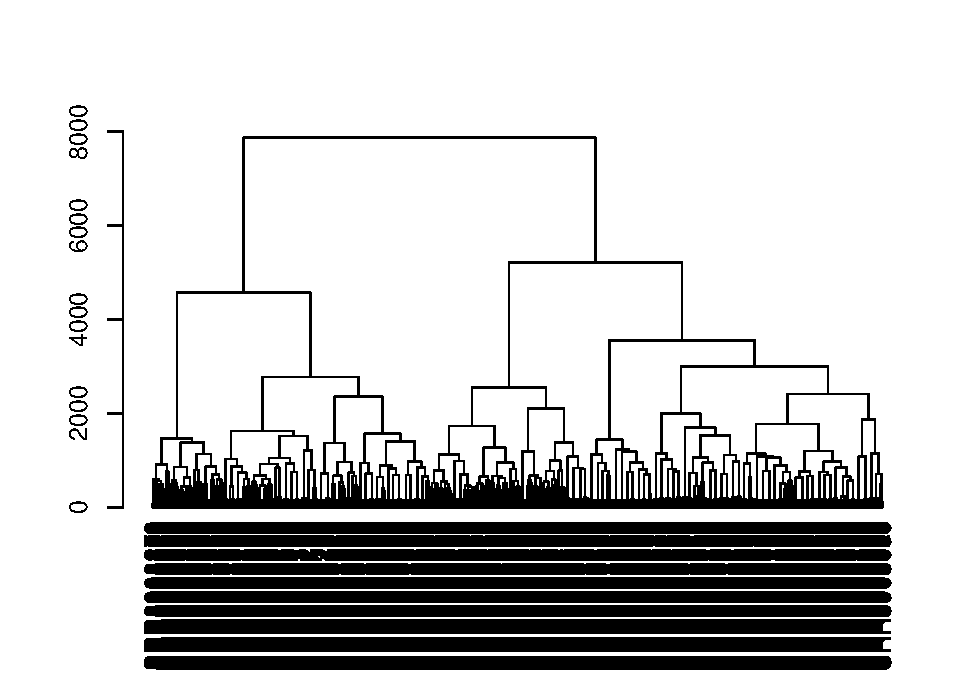
\includegraphics[keepaspectratio]{Assignment3_files/figure-latex/hclust run-1.pdf}}
Above is the plotted dendrogram using Ward hierarchical clustering. This
data is not much use to us as a dendrogram due to the sheer number of
genes. Ideally, we'll represent this data as a heat map. What is useful,
is that we can take the information from the hclust object we created to
determine an optimal number of clusters using the silhouette method,
elbow plot, or gap statatistic.\\

\subsubsection{Number of Clusters}\label{number-of-clusters}

Here we will use information from the \texttt{hclust} object to
determine optimal cluster number using the elbow plot method.\\

\begin{Shaded}
\begin{Highlighting}[]
\FunctionTok{library}\NormalTok{(cluster)}
\FunctionTok{library}\NormalTok{(ggplot2)}
\FunctionTok{library}\NormalTok{(tidyverse)}
\end{Highlighting}
\end{Shaded}

\begin{verbatim}
## -- Attaching core tidyverse packages ------------------------ tidyverse 2.0.0 --
## v forcats   1.0.1     v stringr   1.5.2
## v lubridate 1.9.4     v tidyr     1.3.1
## v purrr     1.1.0     
## -- Conflicts ------------------------------------------ tidyverse_conflicts() --
## x lubridate::%within%()    masks IRanges::%within%()
## x IRanges::collapse()      masks dplyr::collapse()
## x Biobase::combine()       masks BiocGenerics::combine(), dplyr::combine()
## x IRanges::desc()          masks dplyr::desc()
## x tidyr::expand()          masks S4Vectors::expand()
## x dplyr::filter()          masks stats::filter()
## x S4Vectors::first()       masks dplyr::first()
## x dplyr::lag()             masks stats::lag()
## x BiocGenerics::Position() masks ggplot2::Position(), base::Position()
## x purrr::reduce()          masks IRanges::reduce()
## x S4Vectors::rename()      masks dplyr::rename()
## x lubridate::second()      masks S4Vectors::second()
## x lubridate::second<-()    masks S4Vectors::second<-()
## x AnnotationDbi::select()  masks dplyr::select()
## x IRanges::slice()         masks dplyr::slice()
## i Use the conflicted package (<http://conflicted.r-lib.org/>) to force all conflicts to become errors
\end{verbatim}

\begin{Shaded}
\begin{Highlighting}[]
\CommentTok{\# create hclust\_samples dataframe}
\NormalTok{hclust\_samples\_df }\OtherTok{=}\NormalTok{ hclust\_samples}\SpecialCharTok{$}\NormalTok{height }\SpecialCharTok{\%\textgreater{}\%}
            \FunctionTok{as.tibble}\NormalTok{() }\SpecialCharTok{\%\textgreater{}\%}
            \FunctionTok{add\_column}\NormalTok{(}\AttributeTok{groups =} \FunctionTok{length}\NormalTok{(hclust\_samples}\SpecialCharTok{$}\NormalTok{height)}\SpecialCharTok{:}\DecValTok{1}\NormalTok{) }\SpecialCharTok{\%\textgreater{}\%}
            \FunctionTok{filter}\NormalTok{(groups }\SpecialCharTok{\textless{}=} \DecValTok{250}\NormalTok{)}
\end{Highlighting}
\end{Shaded}

\begin{verbatim}
## Warning: `as.tibble()` was deprecated in tibble 2.0.0.
## i Please use `as_tibble()` instead.
## i The signature and semantics have changed, see `?as_tibble`.
## This warning is displayed once every 8 hours.
## Call `lifecycle::last_lifecycle_warnings()` to see where this warning was
## generated.
\end{verbatim}

\begin{Shaded}
\begin{Highlighting}[]
\NormalTok{hs\_df\_plot }\OtherTok{=} \FunctionTok{ggplot}\NormalTok{(hclust\_samples\_df,}
        \FunctionTok{aes}\NormalTok{(}\AttributeTok{x=}\NormalTok{groups, }\AttributeTok{y=}\NormalTok{value)) }\SpecialCharTok{+}
     \FunctionTok{geom\_point}\NormalTok{(}\AttributeTok{shape=}\StringTok{"."}\NormalTok{) }\SpecialCharTok{+}
     \FunctionTok{geom\_line}\NormalTok{()}
\NormalTok{hs\_df\_plot}
\end{Highlighting}
\end{Shaded}

\pandocbounded{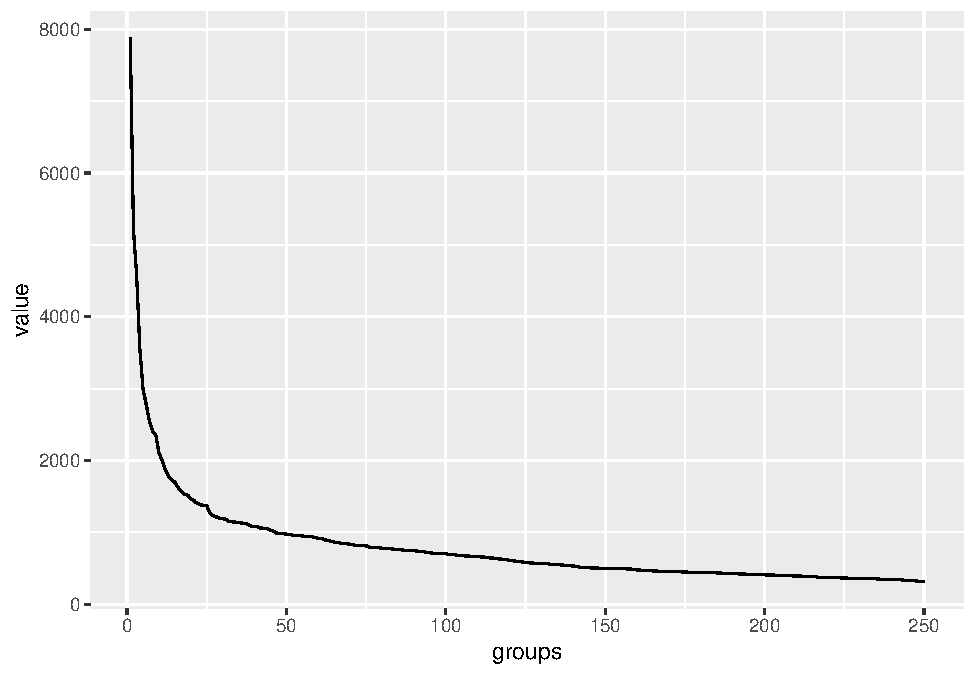
\includegraphics[keepaspectratio]{Assignment3_files/figure-latex/Cluster Determination-1.pdf}}
These elbow plots do not seem very useful. We have too many groups. We
really need to zoom in on the actual elbow to determine the number of
groups we actually need.\\

\begin{Shaded}
\begin{Highlighting}[]
\NormalTok{hs\_df\_plot }\SpecialCharTok{+} 
  \FunctionTok{coord\_cartesian}\NormalTok{(}\AttributeTok{xlim =} \FunctionTok{c}\NormalTok{(}\DecValTok{0}\NormalTok{, }\DecValTok{10}\NormalTok{), }\AttributeTok{ylim =} \FunctionTok{c}\NormalTok{(}\DecValTok{0}\NormalTok{, }\DecValTok{8000}\NormalTok{)) }\SpecialCharTok{+} 
  \CommentTok{\# Add titles and labels}
  \FunctionTok{labs}\NormalTok{(}
    \AttributeTok{title =} \StringTok{"Elbow Plot of"}\NormalTok{,}
    \AttributeTok{x =} \StringTok{"Number of Clusters (k)"}\NormalTok{,}
    \AttributeTok{y =} \StringTok{"Cluster Merge Height (Distance)"}
\NormalTok{  ) }\SpecialCharTok{+}
  \FunctionTok{scale\_color\_brewer}\NormalTok{(}\AttributeTok{palette =} \StringTok{"Dark2"}\NormalTok{) }\SpecialCharTok{+}
  \FunctionTok{theme\_minimal}\NormalTok{(}\AttributeTok{base\_size =} \DecValTok{14}\NormalTok{) }\SpecialCharTok{+}
  
  \CommentTok{\# Draw a vertical line where k=30 (your hypothesized elbow)}
  \FunctionTok{geom\_vline}\NormalTok{(}\AttributeTok{xintercept =} \DecValTok{2}\NormalTok{, }\AttributeTok{linetype =} \StringTok{"dotted"}\NormalTok{, }\AttributeTok{color =} \StringTok{"gray"}\NormalTok{)}
\end{Highlighting}
\end{Shaded}

\pandocbounded{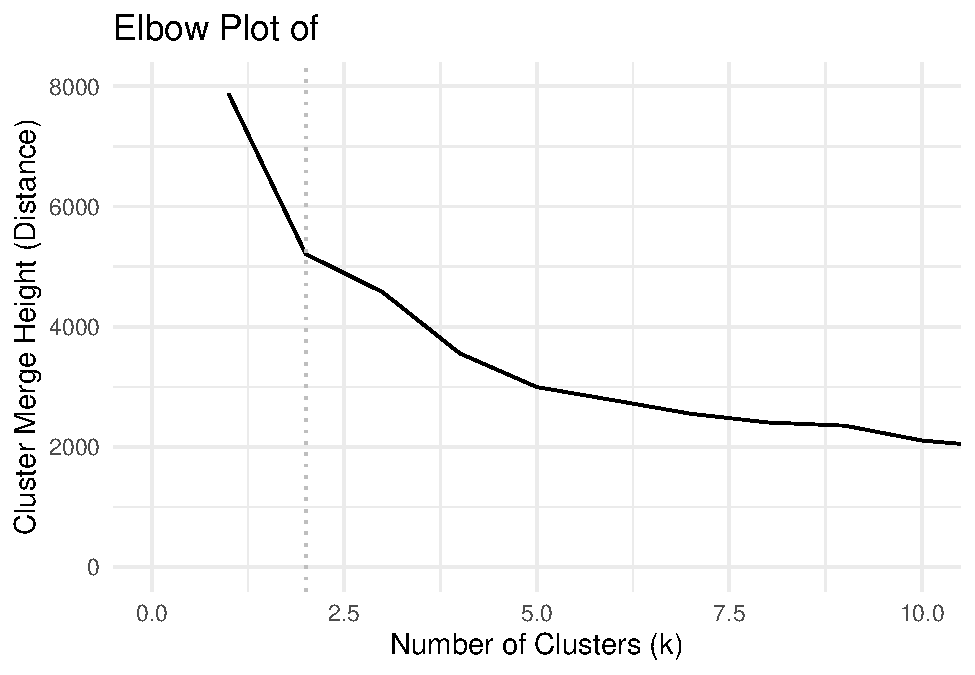
\includegraphics[keepaspectratio]{Assignment3_files/figure-latex/Cluster Determination pt2-1.pdf}}
Our results showed us that there are roughly 30 different groups that
reacted differently to zika virus infection. This suggests that our two
clinical groups, dengue-prior vs dengue-naive, do not behave
statistically differently to zika infection. However, let's perform a
chi-square test to be sure.\\

\subsubsection{Chi-Square Test}\label{chi-square-test}

\begin{Shaded}
\begin{Highlighting}[]
\NormalTok{clusters }\OtherTok{=} \FunctionTok{cutree}\NormalTok{(hclust\_samples, }\AttributeTok{k =} \DecValTok{2}\NormalTok{)}
\CommentTok{\# check if samples match}
\FunctionTok{all}\NormalTok{(}\FunctionTok{sort}\NormalTok{(}\FunctionTok{names}\NormalTok{(clusters)) }\SpecialCharTok{==} \FunctionTok{sort}\NormalTok{(}\FunctionTok{rownames}\NormalTok{(metadata)))}
\end{Highlighting}
\end{Shaded}

\begin{verbatim}
## [1] TRUE
\end{verbatim}

\begin{Shaded}
\begin{Highlighting}[]
\CommentTok{\# check if sample order match}
\FunctionTok{all}\NormalTok{(}\FunctionTok{names}\NormalTok{(clusters) }\SpecialCharTok{==} \FunctionTok{rownames}\NormalTok{(metadata))}
\end{Highlighting}
\end{Shaded}

\begin{verbatim}
## [1] TRUE
\end{verbatim}

\begin{Shaded}
\begin{Highlighting}[]
\NormalTok{contingency\_table }\OtherTok{=} \FunctionTok{table}\NormalTok{(}
  \AttributeTok{Patient\_Groups =}\NormalTok{ clusters,}
  \AttributeTok{Patient\_Exposure =}\NormalTok{ metadata}\SpecialCharTok{$}\NormalTok{Exposure}
\NormalTok{)}

\NormalTok{hs\_cs\_results }\OtherTok{=} \FunctionTok{chisq.test}\NormalTok{(contingency\_table)}
\NormalTok{hs\_cs\_results}
\end{Highlighting}
\end{Shaded}

\begin{verbatim}
## 
##  Pearson's Chi-squared test with Yates' continuity correction
## 
## data:  contingency_table
## X-squared = 4.9444, df = 1, p-value = 0.02617
\end{verbatim}

\begin{Shaded}
\begin{Highlighting}[]
\NormalTok{contingency\_table}
\end{Highlighting}
\end{Shaded}

\begin{verbatim}
##               Patient_Exposure
## Patient_Groups DENV naive
##              1  272   360
##              2  196   193
\end{verbatim}

The chi-square with 2 different clusters suggests that we reject the
null hypothesis that the relationship between dengue virus infection and
subsequent zika infection is independent. At a glance, it may seem that
the proportions are relatively similar, however it should be noted that
there are 553 (\textasciitilde54\%) naive patients out of the 1021
patient samples. This means that there should roughly be a 54\%
proportion of prior dengue infection to naive patients between groups,
however we can see that is not the case with group 2. Here, there is a
higher proportion of DENV patients. A logical follow-up would be to
return to the differential gene expression analysis and investigate the
actual gene pathways involved with this statistical difference with a
new perspective.\\

\begin{Shaded}
\begin{Highlighting}[]
\FunctionTok{library}\NormalTok{(tidyverse)}
\end{Highlighting}
\end{Shaded}

\begin{verbatim}
## -- Attaching core tidyverse packages ------------------------ tidyverse 2.0.0 --
## v forcats   1.0.1     v stringr   1.5.2
## v lubridate 1.9.4     v tidyr     1.3.1
## v purrr     1.1.0     
## -- Conflicts ------------------------------------------ tidyverse_conflicts() --
## x lubridate::%within%()    masks IRanges::%within%()
## x IRanges::collapse()      masks dplyr::collapse()
## x Biobase::combine()       masks BiocGenerics::combine(), dplyr::combine()
## x IRanges::desc()          masks dplyr::desc()
## x tidyr::expand()          masks S4Vectors::expand()
## x dplyr::filter()          masks stats::filter()
## x S4Vectors::first()       masks dplyr::first()
## x dplyr::lag()             masks stats::lag()
## x BiocGenerics::Position() masks ggplot2::Position(), base::Position()
## x purrr::reduce()          masks IRanges::reduce()
## x S4Vectors::rename()      masks dplyr::rename()
## x lubridate::second()      masks S4Vectors::second()
## x lubridate::second<-()    masks S4Vectors::second<-()
## x AnnotationDbi::select()  masks dplyr::select()
## x IRanges::slice()         masks dplyr::slice()
## i Use the conflicted package (<http://conflicted.r-lib.org/>) to force all conflicts to become errors
\end{verbatim}

\begin{Shaded}
\begin{Highlighting}[]
\FunctionTok{library}\NormalTok{(cluster) }\CommentTok{\# for hclust}
\FunctionTok{library}\NormalTok{(matrixStats) }\CommentTok{\# for fast variance calculation}
\end{Highlighting}
\end{Shaded}

\begin{verbatim}
## 
## Attaching package: 'matrixStats'
## 
## The following objects are masked from 'package:Biobase':
## 
##     anyMissing, rowMedians
## 
## The following object is masked from 'package:dplyr':
## 
##     count
\end{verbatim}

\begin{Shaded}
\begin{Highlighting}[]
\NormalTok{gene\_counts\_to\_test }\OtherTok{\textless{}{-}} \FunctionTok{c}\NormalTok{(}\DecValTok{10}\NormalTok{, }\DecValTok{100}\NormalTok{, }\DecValTok{1000}\NormalTok{, }\DecValTok{5000}\NormalTok{)}
\NormalTok{total\_genes }\OtherTok{\textless{}{-}} \FunctionTok{length}\NormalTok{(gene\_vars) }\CommentTok{\# from earlier top 5000 filter}
\NormalTok{gene\_counts\_to\_test }\OtherTok{\textless{}{-}}\NormalTok{ gene\_counts\_to\_test[gene\_counts\_to\_test }\SpecialCharTok{\textless{}=}\NormalTok{ total\_genes]}
\NormalTok{all\_elbow\_data }\OtherTok{\textless{}{-}} \FunctionTok{list}\NormalTok{()}

\ControlFlowTok{for}\NormalTok{ (n\_genes }\ControlFlowTok{in}\NormalTok{ gene\_counts\_to\_test) \{}
 
\NormalTok{  top\_idx }\OtherTok{\textless{}{-}} \FunctionTok{head}\NormalTok{(}\FunctionTok{order}\NormalTok{(gene\_vars, }\AttributeTok{decreasing =} \ConstantTok{TRUE}\NormalTok{), n\_genes)}
\NormalTok{  expression\_filtered }\OtherTok{\textless{}{-}}\NormalTok{ expression\_mat[top\_idx, , drop }\OtherTok{=} \ConstantTok{FALSE}\NormalTok{]}
 
\NormalTok{  dist\_samples }\OtherTok{\textless{}{-}} \FunctionTok{dist}\NormalTok{(}\FunctionTok{t}\NormalTok{(expression\_filtered), }\AttributeTok{method =} \StringTok{"euclidean"}\NormalTok{)}
\NormalTok{  hclust\_samples }\OtherTok{\textless{}{-}} \FunctionTok{hclust}\NormalTok{(dist\_samples, }\AttributeTok{method =} \StringTok{"ward.D2"}\NormalTok{)}
 
\NormalTok{  elbow\_data\_df }\OtherTok{\textless{}{-}} \FunctionTok{data.frame}\NormalTok{(}
    \AttributeTok{height =}\NormalTok{ hclust\_samples}\SpecialCharTok{$}\NormalTok{height,}
    \AttributeTok{groups =}\NormalTok{ (}\FunctionTok{length}\NormalTok{(hclust\_samples}\SpecialCharTok{$}\NormalTok{height) }\SpecialCharTok{+} \DecValTok{1}\NormalTok{)}\SpecialCharTok{:}\DecValTok{2}\NormalTok{,}
    \AttributeTok{Gene\_Count =} \FunctionTok{factor}\NormalTok{(}\FunctionTok{paste0}\NormalTok{(}\StringTok{"Top "}\NormalTok{, n\_genes, }\StringTok{" Genes"}\NormalTok{))}
\NormalTok{  )}
  \CommentTok{\# ignore k values that are too large (helps with computation)}
\NormalTok{  elbow\_data\_df }\OtherTok{\textless{}{-}}\NormalTok{ elbow\_data\_df }\SpecialCharTok{\%\textgreater{}\%} \FunctionTok{filter}\NormalTok{(groups }\SpecialCharTok{\textless{}=} \DecValTok{250}\NormalTok{)}
  
\NormalTok{  all\_elbow\_data[[}\FunctionTok{as.character}\NormalTok{(n\_genes)]] }\OtherTok{\textless{}{-}}\NormalTok{ elbow\_data\_df}
\NormalTok{\}}

\NormalTok{final\_elbow\_df }\OtherTok{\textless{}{-}} \FunctionTok{bind\_rows}\NormalTok{(all\_elbow\_data)}

\CommentTok{\# Generate the comparison ggplot}
\NormalTok{p\_comparison }\OtherTok{\textless{}{-}} \FunctionTok{ggplot}\NormalTok{(final\_elbow\_df, }\FunctionTok{aes}\NormalTok{(}\AttributeTok{x =}\NormalTok{ groups, }\AttributeTok{y =}\NormalTok{ height, }\AttributeTok{color =}\NormalTok{ Gene\_Count)) }\SpecialCharTok{+}
  \FunctionTok{geom\_line}\NormalTok{(}\AttributeTok{linewidth =} \FloatTok{0.8}\NormalTok{) }\SpecialCharTok{+}
  \FunctionTok{geom\_point}\NormalTok{(}\AttributeTok{size =} \FloatTok{0.5}\NormalTok{) }\SpecialCharTok{+}
  
  \CommentTok{\# Zoom in to the relevant elbow area}
  \FunctionTok{coord\_cartesian}\NormalTok{(}\AttributeTok{xlim =} \FunctionTok{c}\NormalTok{(}\DecValTok{1}\NormalTok{, }\DecValTok{10}\NormalTok{), }\AttributeTok{ylim =} \FunctionTok{c}\NormalTok{(}\DecValTok{0}\NormalTok{, }\DecValTok{8000}\NormalTok{)) }\SpecialCharTok{+} 
  
  \CommentTok{\# Add titles and labels}
  \FunctionTok{labs}\NormalTok{(}
    \AttributeTok{title =} \StringTok{"Comparison of Elbow Plots by Gene Feature Count"}\NormalTok{,}
    \AttributeTok{subtitle =} \StringTok{"Assessing the impact of feature selection on patient cluster number (k)"}\NormalTok{,}
    \AttributeTok{x =} \StringTok{"Number of Clusters (k)"}\NormalTok{,}
    \AttributeTok{y =} \StringTok{"Cluster Merge Height (Distance)"}\NormalTok{,}
    \AttributeTok{color =} \StringTok{"Genes Included"}
\NormalTok{  ) }\SpecialCharTok{+}
  \FunctionTok{scale\_color\_brewer}\NormalTok{(}\AttributeTok{palette =} \StringTok{"Dark2"}\NormalTok{) }\SpecialCharTok{+}
  \FunctionTok{theme\_minimal}\NormalTok{(}\AttributeTok{base\_size =} \DecValTok{14}\NormalTok{) }\SpecialCharTok{+}
  
  \CommentTok{\# Draw a vertical line where k=30 (your hypothesized elbow)}
  \FunctionTok{geom\_vline}\NormalTok{(}\AttributeTok{xintercept =} \DecValTok{2}\NormalTok{, }\AttributeTok{linetype =} \StringTok{"dotted"}\NormalTok{, }\AttributeTok{color =} \StringTok{"gray"}\NormalTok{)}

\FunctionTok{print}\NormalTok{(p\_comparison)}
\end{Highlighting}
\end{Shaded}

\pandocbounded{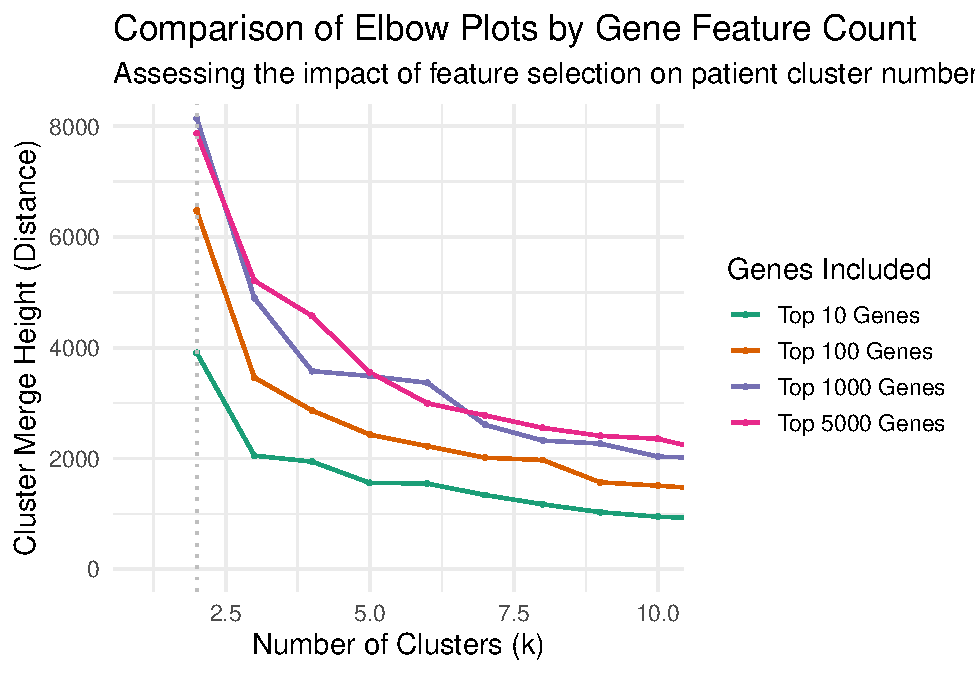
\includegraphics[keepaspectratio]{Assignment3_files/figure-latex/Cluster Determination pt3-1.pdf}}
As we can see here, changing the number of top variable genes does not
change the number of resulting clusters very significantly. This
suggests that the patients relatively set in 2 clusters.\\
\#\#\# Heat Map

\begin{Shaded}
\begin{Highlighting}[]
\FunctionTok{library}\NormalTok{(ComplexHeatmap)}
\end{Highlighting}
\end{Shaded}

\begin{verbatim}
## Loading required package: grid
\end{verbatim}

\begin{verbatim}
## ========================================
## ComplexHeatmap version 2.24.1
## Bioconductor page: http://bioconductor.org/packages/ComplexHeatmap/
## Github page: https://github.com/jokergoo/ComplexHeatmap
## Documentation: http://jokergoo.github.io/ComplexHeatmap-reference
## 
## If you use it in published research, please cite either one:
## - Gu, Z. Complex Heatmap Visualization. iMeta 2022.
## - Gu, Z. Complex heatmaps reveal patterns and correlations in multidimensional 
##     genomic data. Bioinformatics 2016.
## 
## 
## The new InteractiveComplexHeatmap package can directly export static 
## complex heatmaps into an interactive Shiny app with zero effort. Have a try!
## 
## This message can be suppressed by:
##   suppressPackageStartupMessages(library(ComplexHeatmap))
## ========================================
\end{verbatim}

\begin{Shaded}
\begin{Highlighting}[]
\FunctionTok{library}\NormalTok{(magick)}
\end{Highlighting}
\end{Shaded}

\begin{verbatim}
## Warning: package 'magick' was built under R version 4.5.2
\end{verbatim}

\begin{verbatim}
## Linking to ImageMagick 6.9.13.29
## Enabled features: cairo, freetype, fftw, ghostscript, heic, lcms, pango, raw, rsvg, webp
## Disabled features: fontconfig, x11
\end{verbatim}

\begin{Shaded}
\begin{Highlighting}[]
\FunctionTok{library}\NormalTok{(Cairo)}
\end{Highlighting}
\end{Shaded}

\begin{verbatim}
## Warning: package 'Cairo' was built under R version 4.5.2
\end{verbatim}

\begin{Shaded}
\begin{Highlighting}[]
\FunctionTok{gc}\NormalTok{()}
\end{Highlighting}
\end{Shaded}

\begin{verbatim}
##             used  (Mb) gc trigger   (Mb)  max used   (Mb)
## Ncells   5001744 267.2    8857027  473.1   8857027  473.1
## Vcells 108452045 827.5  197005002 1503.1 184032565 1404.1
\end{verbatim}

\begin{Shaded}
\begin{Highlighting}[]
\NormalTok{heatmap }\OtherTok{\textless{}{-}} \FunctionTok{Heatmap}\NormalTok{(}
\NormalTok{    expression\_top5000,}
    \AttributeTok{use\_raster =} \ConstantTok{TRUE}\NormalTok{,}
    \AttributeTok{raster\_by\_magick =} \ConstantTok{TRUE}\NormalTok{,}
    \AttributeTok{raster\_quality =} \DecValTok{1}\NormalTok{,}
    \AttributeTok{cluster\_rows =} \ConstantTok{FALSE}\NormalTok{,}
    \AttributeTok{cluster\_columns =} \ConstantTok{TRUE}\NormalTok{,}
    \AttributeTok{top\_annotation =} \FunctionTok{HeatmapAnnotation}\NormalTok{(}
        \AttributeTok{Dengue\_Status =}\NormalTok{ metadata}\SpecialCharTok{$}\NormalTok{Exposure }
\NormalTok{    ),}
    
    \AttributeTok{column\_title =} \FunctionTok{paste0}\NormalTok{(}\StringTok{"Patient Clustering Axis: Molecular Subtypes (k=2) by Prior Dengue Status (N="}\NormalTok{, }\FunctionTok{ncol}\NormalTok{(expression\_top5000), }\StringTok{")"}\NormalTok{),}
    \AttributeTok{column\_title\_gp =} \FunctionTok{gpar}\NormalTok{(}\AttributeTok{fontsize =} \DecValTok{18}\NormalTok{, }\AttributeTok{fontface =} \StringTok{"bold"}\NormalTok{), }\CommentTok{\# Enhanced Title}
    
    \AttributeTok{row\_title =} \FunctionTok{paste0}\NormalTok{(}\StringTok{"Gene Clustering Axis: 5000 Most Variable Genes"}\NormalTok{),}
    \AttributeTok{row\_title\_rot =} \DecValTok{90}\NormalTok{,}
    \AttributeTok{row\_title\_gp =} \FunctionTok{gpar}\NormalTok{(}\AttributeTok{fontsize =} \DecValTok{18}\NormalTok{, }\AttributeTok{fontface =} \StringTok{"bold"}\NormalTok{), }\CommentTok{\# Enhanced Title}
    
    \AttributeTok{show\_row\_names =} \ConstantTok{FALSE}\NormalTok{,}
    \AttributeTok{show\_column\_names =} \ConstantTok{FALSE}\NormalTok{,}
    
    \AttributeTok{heatmap\_legend\_param =} \FunctionTok{list}\NormalTok{(}
        \AttributeTok{title =} \StringTok{"Log2 Expression (Z{-}score)"}\NormalTok{,}
        \AttributeTok{title\_position =} \StringTok{"topcenter"}\NormalTok{,}
        \AttributeTok{title\_gp =} \FunctionTok{gpar}\NormalTok{(}\AttributeTok{fontsize =} \DecValTok{14}\NormalTok{, }\AttributeTok{fontface =} \StringTok{"bold"}\NormalTok{),}
        \AttributeTok{legend\_direction =} \StringTok{"horizontal"}
\NormalTok{    )}
\NormalTok{)}
\end{Highlighting}
\end{Shaded}

\begin{verbatim}
## The automatically generated colors map from the 1^st and 99^th of the
## values in the matrix. There are outliers in the matrix whose patterns
## might be hidden by this color mapping. You can manually set the color
## to `col` argument.
## 
## Use `suppressMessages()` to turn off this message.
\end{verbatim}

\begin{Shaded}
\begin{Highlighting}[]
\FunctionTok{CairoPDF}\NormalTok{(}\StringTok{"plots/hclust\_patient\_heatmap.pdf"}\NormalTok{, }\AttributeTok{width =} \DecValTok{18}\NormalTok{, }\AttributeTok{height =} \DecValTok{25}\NormalTok{)}
\FunctionTok{draw}\NormalTok{(heatmap)}
\FunctionTok{dev.off}\NormalTok{()}
\end{Highlighting}
\end{Shaded}

\begin{verbatim}
## pdf 
##   2
\end{verbatim}

\subsection{Nikhil Sangamkar: PAM
Clustering}\label{nikhil-sangamkar-pam-clustering}

\begin{Shaded}
\begin{Highlighting}[]
\FunctionTok{suppressPackageStartupMessages}\NormalTok{(\{}
  \FunctionTok{library}\NormalTok{(cluster)}
  \FunctionTok{library}\NormalTok{(glue)}
  \FunctionTok{library}\NormalTok{(dplyr)}
  \FunctionTok{library}\NormalTok{(purrr)}
  \FunctionTok{library}\NormalTok{(tibble)}
\NormalTok{\})}

\FunctionTok{stopifnot}\NormalTok{(}\FunctionTok{exists}\NormalTok{(}\StringTok{"expression\_top5000"}\NormalTok{), }\FunctionTok{exists}\NormalTok{(}\StringTok{"metadata"}\NormalTok{))}

\CommentTok{\# {-}{-}{-} Data prep {-}{-}{-}}
\NormalTok{X\_5000 }\OtherTok{\textless{}{-}} \FunctionTok{t}\NormalTok{(expression\_top5000)        }\CommentTok{\# samples as rows}
\NormalTok{X\_scaled }\OtherTok{\textless{}{-}} \FunctionTok{scale}\NormalTok{(X\_5000)}
\NormalTok{X\_scaled[}\FunctionTok{is.na}\NormalTok{(X\_scaled)] }\OtherTok{\textless{}{-}} \DecValTok{0}

\CommentTok{\# \# range of k values}
\CommentTok{\# k\_values \textless{}{-} 2:8}
\CommentTok{\# pam\_results \textless{}{-} list()}

\CommentTok{\# for (k in k\_values) \{}
\CommentTok{\#   cat(glue("Running PAM with k = \{k\}\textbackslash{}n"))}
\CommentTok{\#   pam\_fit \textless{}{-} pam(X\_scaled, k = k)}
\CommentTok{\#   sil \textless{}{-} silhouette(pam\_fit$clustering, dist(X\_scaled))}
\CommentTok{\#   avg\_sil \textless{}{-} mean(sil[, 3])}
  
\CommentTok{\#   pam\_results[[as.character(k)]] \textless{}{-} list(}
\CommentTok{\#     k = k,}
\CommentTok{\#     pam\_fit = pam\_fit,}
\CommentTok{\#     clusters = pam\_fit$clustering,}
\CommentTok{\#     avg\_silhouette = avg\_sil}
\CommentTok{\#   )}
\CommentTok{\# \}}


\CommentTok{\# summarize silhouette scores}
\NormalTok{pam\_summary }\OtherTok{\textless{}{-}} \FunctionTok{map\_dfr}\NormalTok{(pam\_results, }\ControlFlowTok{function}\NormalTok{(x) \{}
  \FunctionTok{tibble}\NormalTok{(}\AttributeTok{k =} \FunctionTok{as.numeric}\NormalTok{(x}\SpecialCharTok{$}\NormalTok{k), }\AttributeTok{avg\_silhouette =} \FunctionTok{as.numeric}\NormalTok{(x}\SpecialCharTok{$}\NormalTok{avg\_silhouette))}
\NormalTok{\})}
\FunctionTok{print}\NormalTok{(pam\_summary)}

\NormalTok{best\_k }\OtherTok{\textless{}{-}}\NormalTok{ pam\_summary }\SpecialCharTok{\%\textgreater{}\%}
  \FunctionTok{arrange}\NormalTok{(}\FunctionTok{desc}\NormalTok{(avg\_silhouette)) }\SpecialCharTok{\%\textgreater{}\%}
  \FunctionTok{slice\_head}\NormalTok{(}\AttributeTok{n =} \DecValTok{1}\NormalTok{) }\SpecialCharTok{\%\textgreater{}\%}
  \FunctionTok{pull}\NormalTok{(k)}

\FunctionTok{cat}\NormalTok{(}\FunctionTok{glue}\NormalTok{(}\StringTok{"}\SpecialCharTok{\textbackslash{}n}\StringTok{Best k chosen for PAM: \{best\_k\}}\SpecialCharTok{\textbackslash{}n}\StringTok{"}\NormalTok{))}

\NormalTok{pam\_clusters }\OtherTok{\textless{}{-}}\NormalTok{ pam\_results[[}\FunctionTok{as.character}\NormalTok{(best\_k)]]}\SpecialCharTok{$}\NormalTok{clusters}

\NormalTok{gene\_counts }\OtherTok{\textless{}{-}} \FunctionTok{c}\NormalTok{(}\DecValTok{10}\NormalTok{, }\DecValTok{100}\NormalTok{, }\DecValTok{1000}\NormalTok{)}
\FunctionTok{cat}\NormalTok{(}\StringTok{"Running gene\_counts ="}\NormalTok{, }\FunctionTok{paste}\NormalTok{(gene\_counts, }\AttributeTok{collapse =} \StringTok{", "}\NormalTok{), }\StringTok{"}\SpecialCharTok{\textbackslash{}n}\StringTok{"}\NormalTok{)}


\NormalTok{pam\_multi\_results }\OtherTok{\textless{}{-}} \FunctionTok{list}\NormalTok{()}

\ControlFlowTok{for}\NormalTok{ (n\_genes }\ControlFlowTok{in}\NormalTok{ gene\_counts) \{}
  \FunctionTok{cat}\NormalTok{(}\FunctionTok{glue}\NormalTok{(}\StringTok{"}\SpecialCharTok{\textbackslash{}n}\StringTok{{-}{-}{-} Running PAM on top \{n\_genes\} genes {-}{-}{-}}\SpecialCharTok{\textbackslash{}n}\StringTok{"}\NormalTok{))}

  \CommentTok{\# Select top variable genes}
\NormalTok{  gene\_vars }\OtherTok{\textless{}{-}}\NormalTok{ matrixStats}\SpecialCharTok{::}\FunctionTok{rowVars}\NormalTok{(expression\_mat)}
\NormalTok{  top\_idx }\OtherTok{\textless{}{-}} \FunctionTok{head}\NormalTok{(}\FunctionTok{order}\NormalTok{(gene\_vars, }\AttributeTok{decreasing =} \ConstantTok{TRUE}\NormalTok{), n\_genes)}
\NormalTok{  expr\_subset }\OtherTok{\textless{}{-}}\NormalTok{ expression\_mat[top\_idx, , drop }\OtherTok{=} \ConstantTok{FALSE}\NormalTok{]}

  \CommentTok{\# Scale and transpose}
\NormalTok{  X }\OtherTok{\textless{}{-}} \FunctionTok{t}\NormalTok{(expr\_subset)}
\NormalTok{  X\_scaled }\OtherTok{\textless{}{-}} \FunctionTok{scale}\NormalTok{(X)}
\NormalTok{  X\_scaled[}\FunctionTok{is.na}\NormalTok{(X\_scaled)] }\OtherTok{\textless{}{-}} \DecValTok{0}

  \CommentTok{\# PAM clustering for k = 2–8}
\NormalTok{  k\_values }\OtherTok{\textless{}{-}} \DecValTok{2}\SpecialCharTok{:}\DecValTok{8}
\NormalTok{  results\_this\_set }\OtherTok{\textless{}{-}} \FunctionTok{list}\NormalTok{()}

  \ControlFlowTok{for}\NormalTok{ (k }\ControlFlowTok{in}\NormalTok{ k\_values) \{}
\NormalTok{    pam\_fit }\OtherTok{\textless{}{-}} \FunctionTok{pam}\NormalTok{(X\_scaled, }\AttributeTok{k =}\NormalTok{ k)}
\NormalTok{    sil }\OtherTok{\textless{}{-}} \FunctionTok{silhouette}\NormalTok{(pam\_fit}\SpecialCharTok{$}\NormalTok{clustering, }\FunctionTok{dist}\NormalTok{(X\_scaled))}
\NormalTok{    avg\_sil }\OtherTok{\textless{}{-}} \FunctionTok{mean}\NormalTok{(sil[, }\DecValTok{3}\NormalTok{])}

\NormalTok{    results\_this\_set[[}\FunctionTok{as.character}\NormalTok{(k)]] }\OtherTok{\textless{}{-}} \FunctionTok{list}\NormalTok{(}
      \AttributeTok{k =}\NormalTok{ k,}
      \AttributeTok{clusters =}\NormalTok{ pam\_fit}\SpecialCharTok{$}\NormalTok{clustering,}
      \AttributeTok{avg\_sil =}\NormalTok{ avg\_sil}
\NormalTok{    )}
\NormalTok{  \}}

  \CommentTok{\# pick best k by silhouette}
\NormalTok{  sil\_df }\OtherTok{\textless{}{-}} \FunctionTok{map\_dfr}\NormalTok{(results\_this\_set, }\SpecialCharTok{\textasciitilde{}}\FunctionTok{tibble}\NormalTok{(}\AttributeTok{k =}\NormalTok{ .x}\SpecialCharTok{$}\NormalTok{k, }\AttributeTok{avg\_sil =}\NormalTok{ .x}\SpecialCharTok{$}\NormalTok{avg\_sil))}
\NormalTok{  best\_k }\OtherTok{\textless{}{-}}\NormalTok{ sil\_df }\SpecialCharTok{\%\textgreater{}\%} \FunctionTok{arrange}\NormalTok{(}\FunctionTok{desc}\NormalTok{(avg\_sil)) }\SpecialCharTok{\%\textgreater{}\%} \FunctionTok{slice\_head}\NormalTok{(}\AttributeTok{n =} \DecValTok{1}\NormalTok{) }\SpecialCharTok{\%\textgreater{}\%} \FunctionTok{pull}\NormalTok{(k)}

  \FunctionTok{cat}\NormalTok{(}\FunctionTok{glue}\NormalTok{(}\StringTok{"Best k = \{best\_k\} (silhouette = \{round(max(sil\_df$avg\_sil), 3)\})}\SpecialCharTok{\textbackslash{}n}\StringTok{"}\NormalTok{))}

  \CommentTok{\# Chi{-}squared test vs. exposure groups}
\NormalTok{  clusters }\OtherTok{\textless{}{-}}\NormalTok{ results\_this\_set[[}\FunctionTok{as.character}\NormalTok{(best\_k)]]}\SpecialCharTok{$}\NormalTok{clusters}
\NormalTok{  exposures }\OtherTok{\textless{}{-}}\NormalTok{ metadata}\SpecialCharTok{$}\NormalTok{Exposure}
  \FunctionTok{names}\NormalTok{(exposures) }\OtherTok{\textless{}{-}}\NormalTok{ metadata}\SpecialCharTok{$}\NormalTok{refinebio\_accession\_code}
\NormalTok{  common }\OtherTok{\textless{}{-}} \FunctionTok{intersect}\NormalTok{(}\FunctionTok{names}\NormalTok{(clusters), }\FunctionTok{names}\NormalTok{(exposures))}
\NormalTok{  tab }\OtherTok{\textless{}{-}} \FunctionTok{table}\NormalTok{(}\AttributeTok{Exposure =}\NormalTok{ exposures[common], }\AttributeTok{Cluster =}\NormalTok{ clusters[common])}
\NormalTok{  chi }\OtherTok{\textless{}{-}} \FunctionTok{suppressWarnings}\NormalTok{(}\FunctionTok{chisq.test}\NormalTok{(tab))}

\NormalTok{  pam\_multi\_results[[}\FunctionTok{paste0}\NormalTok{(}\StringTok{"genes\_"}\NormalTok{, n\_genes)]] }\OtherTok{\textless{}{-}} \FunctionTok{list}\NormalTok{(}
    \AttributeTok{n\_genes =}\NormalTok{ n\_genes,}
    \AttributeTok{best\_k =}\NormalTok{ best\_k,}
    \AttributeTok{silhouette =} \FunctionTok{max}\NormalTok{(sil\_df}\SpecialCharTok{$}\NormalTok{avg\_sil),}
    \AttributeTok{chi\_sq =} \FunctionTok{unname}\NormalTok{(chi}\SpecialCharTok{$}\NormalTok{statistic),}
    \AttributeTok{df =} \FunctionTok{unname}\NormalTok{(chi}\SpecialCharTok{$}\NormalTok{parameter),}
    \AttributeTok{p\_value =}\NormalTok{ chi}\SpecialCharTok{$}\NormalTok{p.value}
\NormalTok{  )}
\NormalTok{\}}

\CommentTok{\# Combine into one summary tibble}
\NormalTok{pam\_multi\_summary }\OtherTok{\textless{}{-}} \FunctionTok{bind\_rows}\NormalTok{(}\FunctionTok{lapply}\NormalTok{(pam\_multi\_results, as\_tibble)) }\SpecialCharTok{\%\textgreater{}\%}
  \FunctionTok{mutate}\NormalTok{(}\AttributeTok{adj\_p\_value =} \FunctionTok{p.adjust}\NormalTok{(p\_value, }\AttributeTok{method =} \StringTok{"BH"}\NormalTok{))}

\NormalTok{knitr}\SpecialCharTok{::}\FunctionTok{kable}\NormalTok{(pam\_multi\_summary,}
  \AttributeTok{caption =} \StringTok{"Chi{-}squared test results for PAM clustering across gene subsets"}
\NormalTok{)}

\CommentTok{\# {-}{-}{-} Chi{-}squared test with exposure groups {-}{-}{-}}
\NormalTok{exposures }\OtherTok{\textless{}{-}}\NormalTok{ metadata}\SpecialCharTok{$}\NormalTok{Exposure}
\FunctionTok{names}\NormalTok{(exposures) }\OtherTok{\textless{}{-}}\NormalTok{ metadata}\SpecialCharTok{$}\NormalTok{refinebio\_accession\_code}

\NormalTok{common\_samples }\OtherTok{\textless{}{-}} \FunctionTok{intersect}\NormalTok{(}\FunctionTok{names}\NormalTok{(pam\_clusters), }\FunctionTok{names}\NormalTok{(exposures))}
\NormalTok{tab }\OtherTok{\textless{}{-}} \FunctionTok{table}\NormalTok{(}\AttributeTok{Exposure =}\NormalTok{ exposures[common\_samples],}
             \AttributeTok{Cluster =}\NormalTok{ pam\_clusters[common\_samples])}

\NormalTok{pam\_chi }\OtherTok{\textless{}{-}} \FunctionTok{suppressWarnings}\NormalTok{(}\FunctionTok{chisq.test}\NormalTok{(tab))}
\NormalTok{pam\_chi}

\NormalTok{pam\_clusters\_5000 }\OtherTok{\textless{}{-}} \FunctionTok{tibble}\NormalTok{(}
  \AttributeTok{sample\_id =} \FunctionTok{names}\NormalTok{(pam\_clusters),}
  \AttributeTok{cluster =} \FunctionTok{as.character}\NormalTok{(pam\_clusters)}
\NormalTok{)}
\FunctionTok{assign}\NormalTok{(}\StringTok{"pam\_clusters\_5000"}\NormalTok{, pam\_clusters\_5000, }\AttributeTok{envir =}\NormalTok{ .GlobalEnv)}
\FunctionTok{assign}\NormalTok{(}\StringTok{"pam\_best\_k"}\NormalTok{, best\_k, }\AttributeTok{envir =}\NormalTok{ .GlobalEnv)}

\FunctionTok{table}\NormalTok{(pam\_clusters)}

\CommentTok{\# {-}{-}{-} Heatmap of 5000 genes with PAM clusters {-}{-}{-}}
\FunctionTok{suppressPackageStartupMessages}\NormalTok{(\{}
  \FunctionTok{library}\NormalTok{(ComplexHeatmap)}
  \FunctionTok{library}\NormalTok{(circlize)}
  \FunctionTok{library}\NormalTok{(RColorBrewer)}
  \FunctionTok{library}\NormalTok{(scales)}
\NormalTok{\})}

\NormalTok{heatmap\_matrix }\OtherTok{\textless{}{-}} \FunctionTok{log2}\NormalTok{(expression\_top5000 }\SpecialCharTok{+} \DecValTok{1}\NormalTok{)}
\NormalTok{heatmap\_matrix }\OtherTok{\textless{}{-}} \FunctionTok{t}\NormalTok{(}\FunctionTok{scale}\NormalTok{(}\FunctionTok{t}\NormalTok{(heatmap\_matrix)))}
\NormalTok{heatmap\_matrix[}\SpecialCharTok{!}\FunctionTok{is.finite}\NormalTok{(heatmap\_matrix)] }\OtherTok{\textless{}{-}} \DecValTok{0}
\NormalTok{heatmap\_samples }\OtherTok{\textless{}{-}} \FunctionTok{colnames}\NormalTok{(heatmap\_matrix)}

\NormalTok{pam\_col }\OtherTok{\textless{}{-}}\NormalTok{ pam\_clusters[}\FunctionTok{match}\NormalTok{(heatmap\_samples, }\FunctionTok{names}\NormalTok{(pam\_clusters))]}
\NormalTok{exposure\_col }\OtherTok{\textless{}{-}} \FunctionTok{as.character}\NormalTok{(metadata}\SpecialCharTok{$}\NormalTok{Exposure[}\FunctionTok{match}\NormalTok{(heatmap\_samples, metadata}\SpecialCharTok{$}\NormalTok{refinebio\_accession\_code)])}

\NormalTok{pam\_factor }\OtherTok{\textless{}{-}} \FunctionTok{factor}\NormalTok{(pam\_col)}
\NormalTok{exposure\_factor }\OtherTok{\textless{}{-}} \FunctionTok{factor}\NormalTok{(exposure\_col)}

\NormalTok{ann\_col }\OtherTok{\textless{}{-}} \FunctionTok{HeatmapAnnotation}\NormalTok{(}
  \AttributeTok{Exposure =}\NormalTok{ exposure\_factor,}
  \AttributeTok{PAM =}\NormalTok{ pam\_factor,}
  \AttributeTok{col =} \FunctionTok{list}\NormalTok{(}
    \AttributeTok{Exposure =} \FunctionTok{setNames}\NormalTok{(}\FunctionTok{hue\_pal}\NormalTok{()(}\FunctionTok{length}\NormalTok{(}\FunctionTok{levels}\NormalTok{(exposure\_factor))), }\FunctionTok{levels}\NormalTok{(exposure\_factor)),}
    \AttributeTok{PAM =} \FunctionTok{setNames}\NormalTok{(}\FunctionTok{brewer.pal}\NormalTok{(}\FunctionTok{max}\NormalTok{(}\DecValTok{3}\NormalTok{, }\FunctionTok{length}\NormalTok{(}\FunctionTok{levels}\NormalTok{(pam\_factor))), }\StringTok{"Set2"}\NormalTok{)[}\FunctionTok{seq\_along}\NormalTok{(}\FunctionTok{levels}\NormalTok{(pam\_factor))],}
                   \FunctionTok{levels}\NormalTok{(pam\_factor))}
\NormalTok{  )}
\NormalTok{)}

\NormalTok{pam\_heatmap }\OtherTok{\textless{}{-}} \FunctionTok{Heatmap}\NormalTok{(}
  \AttributeTok{name =} \StringTok{"Z{-}score"}\NormalTok{,}
  \AttributeTok{matrix =}\NormalTok{ heatmap\_matrix,}
  \AttributeTok{cluster\_rows =} \ConstantTok{TRUE}\NormalTok{,}
  \AttributeTok{cluster\_columns =} \ConstantTok{TRUE}\NormalTok{,}
  \AttributeTok{show\_row\_names =} \ConstantTok{FALSE}\NormalTok{,}
  \AttributeTok{show\_column\_names =} \ConstantTok{FALSE}\NormalTok{,}
  \AttributeTok{top\_annotation =}\NormalTok{ ann\_col,}
  \AttributeTok{column\_title =} \FunctionTok{glue}\NormalTok{(}\StringTok{"Top 5000 genes {-} PAM (k = \{best\_k\})"}\NormalTok{),}
  \AttributeTok{row\_title =} \StringTok{"Genes"}
\NormalTok{)}

\FunctionTok{dir.create}\NormalTok{(}\StringTok{"plots"}\NormalTok{, }\AttributeTok{showWarnings =} \ConstantTok{FALSE}\NormalTok{)}
\FunctionTok{pdf}\NormalTok{(}\FunctionTok{file.path}\NormalTok{(}\StringTok{"plots"}\NormalTok{, }\StringTok{"pam\_heatmap\_top5000.pdf"}\NormalTok{), }\AttributeTok{width =} \DecValTok{11}\NormalTok{, }\AttributeTok{height =} \FloatTok{8.5}\NormalTok{)}
\FunctionTok{draw}\NormalTok{(pam\_heatmap, }\AttributeTok{merge\_legend =} \ConstantTok{TRUE}\NormalTok{)}
\FunctionTok{dev.off}\NormalTok{()}

\CommentTok{\# Export cluster assignments for comparison with other methods}
\NormalTok{pam\_clusters\_5000 }\OtherTok{\textless{}{-}} \FunctionTok{tibble}\NormalTok{(}\AttributeTok{sample\_id =} \FunctionTok{names}\NormalTok{(pam\_clusters), }\AttributeTok{cluster =} \FunctionTok{as.character}\NormalTok{(pam\_clusters))}
\FunctionTok{assign}\NormalTok{(}\StringTok{"pam\_clusters\_5000"}\NormalTok{, pam\_clusters\_5000, }\AttributeTok{envir =}\NormalTok{ .GlobalEnv)}
\FunctionTok{assign}\NormalTok{(}\StringTok{"pam\_best\_k"}\NormalTok{, best\_k, }\AttributeTok{envir =}\NormalTok{ .GlobalEnv)}

\FunctionTok{png}\NormalTok{(}\StringTok{"plots/pam\_heatmap\_top5000.png"}\NormalTok{, }\AttributeTok{width =} \DecValTok{2000}\NormalTok{, }\AttributeTok{height =} \DecValTok{1600}\NormalTok{, }\AttributeTok{res =} \DecValTok{250}\NormalTok{)}
\FunctionTok{draw}\NormalTok{(pam\_heatmap, }\AttributeTok{merge\_legend =} \ConstantTok{TRUE}\NormalTok{)}
\FunctionTok{dev.off}\NormalTok{()}
\FunctionTok{browseURL}\NormalTok{(}\StringTok{"plots/pam\_heatmap\_top5000.pdf"}\NormalTok{)}
\end{Highlighting}
\end{Shaded}

I applied Partitioning Around Medoids (PAM) clustering to the top 5000
most variable genes, testing k values from 2 to 8. The average
silhouette width was highest for k = 2 (0.099), indicating two primary
sample groups. T his aligns with the k-means results but with lower
sensitivity to outliers due to PAM's medoid-based approach. The clusters
contained 676 and 345 samples, respectively. When k increased beyond 2,
the silhouette scores decreased at a steady rate, and it seemed that
additional clusters were not biologically meaningful in terms of
results. Specificaly, the silhouette scores went from 0.999 at k = 2 to
0.065 at k = 8, showing that the clusters became less distinct. So, I
chose k = 2 samples to strike the optimal balance. I then reran PAM with
10, 100, 1000, and 10000 genes, which took varying amounts of time, but
the k value of 2 stayed consistent. With small gene sets, the cluster
boundaries were more unstable, and with larger sets, the clusters
stabilized. I also performed chi-squared tests; here is the table Table:
Chi-squared test results for PAM clustering across gene subsets

{\def\LTcaptype{none} % do not increment counter
\begin{longtable}[]{@{}rrrrrrr@{}}
\toprule\noalign{}
n\_genes & best\_k & silhouette & chi\_sq & df & p\_value &
adj\_p\_value \\
\midrule\noalign{}
\endhead
\bottomrule\noalign{}
\endlastfoot
10 & 2 & 0.3492291 & 25.8886644 & 1 & 0.0000004 & 0.0000014 \\
100 & 2 & 0.2491895 & 0.9447949 & 1 & 0.3310478 & 0.3310478 \\
1000 & 2 & 0.1407231 & 14.1447630 & 1 & 0.0001693 & 0.0002257 \\
10000 & 2 & 0.0735371 & 16.6772980 & 1 & 0.0000443 & 0.0000886 \\
\end{longtable}
}

This shows that as the number of genes increased, the p values
decreased, except with a very small number of genes, 10 to be exact
where there was not enough data. I also generated a heatmap with
hierarchical row and column dendrograms and annotations for both PAM
clusters (k = 2) and exposure groups from Assignment 1. The z-scored
expression profiles display clear global differences between the two PAM
clusters, though overlap is visible across some samples. After running
PAM for k = 2 -- 8 across the 5 000 most variable genes, k = 2 yielding
the highest average silhouette (≈ 0.10). Repeating the analysis for 10
-- 10 000 genes revealed similar results: silhouette scores declined
gradually as dimensionality increased, but the optimal k remained 2.
Heatmaps of the top 5 000 genes showed two major expression clusters
that partially overlapped with exposure groups. The chi-squared tests
confirmed that these two clusters were statistically associated with
exposure in most gene subsets.

\subsection{Taylor Tillander: K-means
Clustering}\label{taylor-tillander-k-means-clustering}

\begin{Shaded}
\begin{Highlighting}[]
\FunctionTok{suppressPackageStartupMessages}\NormalTok{(\{}
    \FunctionTok{library}\NormalTok{(dplyr)}
    \FunctionTok{library}\NormalTok{(tidyr)}
    \FunctionTok{library}\NormalTok{(purrr)}
    \FunctionTok{library}\NormalTok{(tibble)}
    \FunctionTok{library}\NormalTok{(matrixStats)}
    \FunctionTok{library}\NormalTok{(cluster)}
    \FunctionTok{library}\NormalTok{(forcats)}
    \FunctionTok{library}\NormalTok{(mclust)}
    \FunctionTok{library}\NormalTok{(glue)}
\NormalTok{\})}

\FunctionTok{stopifnot}\NormalTok{(}\FunctionTok{exists}\NormalTok{(}\StringTok{"expression\_mat"}\NormalTok{), }\FunctionTok{exists}\NormalTok{(}\StringTok{"metadata"}\NormalTok{))}

\NormalTok{metadata\_exposure }\OtherTok{\textless{}{-}}\NormalTok{ metadata }\SpecialCharTok{\%\textgreater{}\%}
    \FunctionTok{mutate}\NormalTok{(}
        \AttributeTok{refinebio\_accession\_code =} \FunctionTok{as.character}\NormalTok{(refinebio\_accession\_code),}
        \AttributeTok{Exposure =}\NormalTok{ forcats}\SpecialCharTok{::}\FunctionTok{fct\_na\_value\_to\_level}\NormalTok{(Exposure, }\AttributeTok{level =} \StringTok{"Unknown"}\NormalTok{)}
\NormalTok{    )}

\NormalTok{exposure\_lookup }\OtherTok{\textless{}{-}}\NormalTok{ metadata\_exposure }\SpecialCharTok{\%\textgreater{}\%}
\NormalTok{  dplyr}\SpecialCharTok{::}\FunctionTok{select}\NormalTok{(refinebio\_accession\_code, Exposure) }\SpecialCharTok{\%\textgreater{}\%}
  \FunctionTok{mutate}\NormalTok{(}\AttributeTok{Exposure =} \FunctionTok{as.character}\NormalTok{(Exposure)) }\SpecialCharTok{\%\textgreater{}\%}
  \FunctionTok{deframe}\NormalTok{()}


\NormalTok{exposure\_table }\OtherTok{\textless{}{-}}\NormalTok{ metadata\_exposure }\SpecialCharTok{\%\textgreater{}\%}
\NormalTok{  dplyr}\SpecialCharTok{::}\FunctionTok{transmute}\NormalTok{(}
        \AttributeTok{sample\_id =}\NormalTok{ refinebio\_accession\_code,}
        \AttributeTok{exposure =} \FunctionTok{as.character}\NormalTok{(Exposure)}
\NormalTok{    )}

\NormalTok{k\_grid }\OtherTok{\textless{}{-}} \DecValTok{2}\SpecialCharTok{:}\DecValTok{8}
\NormalTok{kmeans\_seed }\OtherTok{\textless{}{-}} \DecValTok{0}\DataTypeTok{L}

\NormalTok{select\_top\_genes }\OtherTok{\textless{}{-}} \ControlFlowTok{function}\NormalTok{(mat, n) \{}
\NormalTok{    n }\OtherTok{\textless{}{-}} \FunctionTok{min}\NormalTok{(n, }\FunctionTok{nrow}\NormalTok{(mat))}
\NormalTok{    variances }\OtherTok{\textless{}{-}}\NormalTok{ matrixStats}\SpecialCharTok{::}\FunctionTok{rowVars}\NormalTok{(mat)}
\NormalTok{    ordered }\OtherTok{\textless{}{-}} \FunctionTok{order}\NormalTok{(variances, }\AttributeTok{decreasing =} \ConstantTok{TRUE}\NormalTok{)}
\NormalTok{    idx }\OtherTok{\textless{}{-}} \FunctionTok{head}\NormalTok{(ordered, n)}
    \FunctionTok{list}\NormalTok{(}\AttributeTok{idx =}\NormalTok{ idx, }\AttributeTok{genes =} \FunctionTok{rownames}\NormalTok{(mat)[idx], }\AttributeTok{variances =}\NormalTok{ variances[idx])}
\NormalTok{\}}

\NormalTok{compute\_pca\_scores }\OtherTok{\textless{}{-}} \ControlFlowTok{function}\NormalTok{(mat, idx, }\AttributeTok{max\_components =} \DecValTok{50}\NormalTok{) \{}
\NormalTok{    X }\OtherTok{\textless{}{-}} \FunctionTok{t}\NormalTok{(mat[idx, , }\AttributeTok{drop =} \ConstantTok{FALSE}\NormalTok{])}
\NormalTok{    X\_scaled }\OtherTok{\textless{}{-}} \FunctionTok{scale}\NormalTok{(X)}
\NormalTok{    X\_scaled[}\FunctionTok{is.na}\NormalTok{(X\_scaled)] }\OtherTok{\textless{}{-}} \DecValTok{0}
\NormalTok{    pc }\OtherTok{\textless{}{-}} \FunctionTok{prcomp}\NormalTok{(X\_scaled, }\AttributeTok{center =} \ConstantTok{FALSE}\NormalTok{, }\AttributeTok{scale. =} \ConstantTok{FALSE}\NormalTok{)}
    \ControlFlowTok{if}\NormalTok{ (}\FunctionTok{ncol}\NormalTok{(pc}\SpecialCharTok{$}\NormalTok{x) }\SpecialCharTok{==} \DecValTok{0}\NormalTok{) \{}
        \FunctionTok{stop}\NormalTok{(}\StringTok{"PCA returned zero components; check the input variance."}\NormalTok{)}
\NormalTok{    \}}
\NormalTok{    ncomp }\OtherTok{\textless{}{-}} \FunctionTok{min}\NormalTok{(max\_components, }\FunctionTok{ncol}\NormalTok{(pc}\SpecialCharTok{$}\NormalTok{x))}
\NormalTok{    pc}\SpecialCharTok{$}\NormalTok{x[, }\FunctionTok{seq\_len}\NormalTok{(ncomp), drop }\OtherTok{=} \ConstantTok{FALSE}\NormalTok{]}
\NormalTok{\}}

\NormalTok{run\_kmeans\_models }\OtherTok{\textless{}{-}} \ControlFlowTok{function}\NormalTok{(scores, k\_values, }\AttributeTok{seed =}\NormalTok{ kmeans\_seed) \{}
\NormalTok{    dist\_mat }\OtherTok{\textless{}{-}} \FunctionTok{dist}\NormalTok{(scores)}
\NormalTok{    sample\_ids }\OtherTok{\textless{}{-}} \FunctionTok{rownames}\NormalTok{(scores)}
\NormalTok{    purrr}\SpecialCharTok{::}\FunctionTok{map\_dfr}\NormalTok{(k\_values, }\ControlFlowTok{function}\NormalTok{(k) \{}
        \FunctionTok{set.seed}\NormalTok{(seed }\SpecialCharTok{+}\NormalTok{ k)}
\NormalTok{        fit }\OtherTok{\textless{}{-}}\NormalTok{ stats}\SpecialCharTok{::}\FunctionTok{kmeans}\NormalTok{(scores, }\AttributeTok{centers =}\NormalTok{ k, }\AttributeTok{nstart =} \DecValTok{50}\NormalTok{)}
\NormalTok{        clusters }\OtherTok{\textless{}{-}} \FunctionTok{factor}\NormalTok{(fit}\SpecialCharTok{$}\NormalTok{cluster, }\AttributeTok{levels =} \FunctionTok{seq\_len}\NormalTok{(k))}
        \FunctionTok{names}\NormalTok{(clusters) }\OtherTok{\textless{}{-}}\NormalTok{ sample\_ids}
\NormalTok{        sil }\OtherTok{\textless{}{-}}\NormalTok{ cluster}\SpecialCharTok{::}\FunctionTok{silhouette}\NormalTok{(}\FunctionTok{as.integer}\NormalTok{(clusters), dist\_mat)}
        \FunctionTok{tibble}\NormalTok{(}
            \AttributeTok{k =}\NormalTok{ k,}
            \AttributeTok{tot\_withinss =}\NormalTok{ fit}\SpecialCharTok{$}\NormalTok{tot.withinss,}
            \AttributeTok{scaled\_tot\_withinss =}\NormalTok{ fit}\SpecialCharTok{$}\NormalTok{tot.withinss }\SpecialCharTok{/}\NormalTok{ k,}
            \AttributeTok{avg\_silhouette =} \FunctionTok{mean}\NormalTok{(sil[, }\DecValTok{3}\NormalTok{]),}
            \AttributeTok{model =} \FunctionTok{list}\NormalTok{(fit),}
            \AttributeTok{clusters =} \FunctionTok{list}\NormalTok{(clusters),}
            \AttributeTok{silhouette =} \FunctionTok{list}\NormalTok{(sil)}
\NormalTok{        )}
\NormalTok{    \})}
\NormalTok{\}}

\NormalTok{extract\_assignments }\OtherTok{\textless{}{-}} \ControlFlowTok{function}\NormalTok{(models\_tbl) \{}
\NormalTok{    models\_tbl }\SpecialCharTok{\%\textgreater{}\%}
        \FunctionTok{mutate}\NormalTok{(}\AttributeTok{assignment =}\NormalTok{ purrr}\SpecialCharTok{::}\FunctionTok{map}\NormalTok{(clusters, }\SpecialCharTok{\textasciitilde{}} \FunctionTok{tibble}\NormalTok{(}
            \AttributeTok{sample\_id =} \FunctionTok{names}\NormalTok{(.x),}
            \AttributeTok{cluster =} \FunctionTok{as.character}\NormalTok{(.x)}
\NormalTok{        ))) }\SpecialCharTok{\%\textgreater{}\%}
\NormalTok{    dplyr}\SpecialCharTok{::}\FunctionTok{select}\NormalTok{(k, assignment) }\SpecialCharTok{\%\textgreater{}\%}
        \FunctionTok{unnest}\NormalTok{(assignment)}
\NormalTok{\}}

\NormalTok{cluster\_summary }\OtherTok{\textless{}{-}} \ControlFlowTok{function}\NormalTok{(assignments, exposure\_df) \{}
\NormalTok{    assignments }\SpecialCharTok{\%\textgreater{}\%}
        \FunctionTok{mutate}\NormalTok{(}\AttributeTok{cluster =} \FunctionTok{as.character}\NormalTok{(cluster)) }\SpecialCharTok{\%\textgreater{}\%}
        \FunctionTok{left\_join}\NormalTok{(exposure\_df, }\AttributeTok{by =} \StringTok{"sample\_id"}\NormalTok{) }\SpecialCharTok{\%\textgreater{}\%}
        \FunctionTok{mutate}\NormalTok{(}\AttributeTok{exposure =} \FunctionTok{ifelse}\NormalTok{(}\FunctionTok{is.na}\NormalTok{(exposure), }\StringTok{"Unknown"}\NormalTok{, exposure)) }\SpecialCharTok{\%\textgreater{}\%}
        \FunctionTok{group\_by}\NormalTok{(k, cluster, exposure) }\SpecialCharTok{\%\textgreater{}\%}
        \FunctionTok{summarise}\NormalTok{(}\AttributeTok{n =}\NormalTok{ dplyr}\SpecialCharTok{::}\FunctionTok{n}\NormalTok{(), }\AttributeTok{.groups =} \StringTok{"drop\_last"}\NormalTok{) }\SpecialCharTok{\%\textgreater{}\%}
        \FunctionTok{mutate}\NormalTok{(}\AttributeTok{cluster\_total =} \FunctionTok{sum}\NormalTok{(n)) }\SpecialCharTok{\%\textgreater{}\%}
        \FunctionTok{arrange}\NormalTok{(}\FunctionTok{desc}\NormalTok{(n), }\AttributeTok{.by\_group =} \ConstantTok{TRUE}\NormalTok{) }\SpecialCharTok{\%\textgreater{}\%}
\NormalTok{    dplyr}\SpecialCharTok{::}\FunctionTok{slice}\NormalTok{(}\DecValTok{1}\DataTypeTok{L}\NormalTok{) }\SpecialCharTok{\%\textgreater{}\%}
        \FunctionTok{ungroup}\NormalTok{() }\SpecialCharTok{\%\textgreater{}\%}
\NormalTok{    dplyr}\SpecialCharTok{::}\FunctionTok{transmute}\NormalTok{(}
\NormalTok{            k,}
            \AttributeTok{cluster =} \FunctionTok{factor}\NormalTok{(cluster),}
            \AttributeTok{samples\_in\_cluster =}\NormalTok{ cluster\_total,}
            \AttributeTok{majority\_exposure =}\NormalTok{ exposure,}
            \AttributeTok{majority\_fraction =} \FunctionTok{round}\NormalTok{(n }\SpecialCharTok{/}\NormalTok{ cluster\_total, }\DecValTok{3}\NormalTok{)}
\NormalTok{        )}
\NormalTok{\}}

\NormalTok{pairwise\_ari }\OtherTok{\textless{}{-}} \ControlFlowTok{function}\NormalTok{(assignments) \{}
\NormalTok{    k\_vals }\OtherTok{\textless{}{-}} \FunctionTok{sort}\NormalTok{(}\FunctionTok{unique}\NormalTok{(assignments}\SpecialCharTok{$}\NormalTok{k))}
    \ControlFlowTok{if}\NormalTok{ (}\FunctionTok{length}\NormalTok{(k\_vals) }\SpecialCharTok{\textless{}} \DecValTok{2}\NormalTok{) \{}
        \FunctionTok{return}\NormalTok{(}\FunctionTok{tibble}\NormalTok{())}
\NormalTok{    \}}
    \FunctionTok{combn}\NormalTok{(k\_vals, }\DecValTok{2}\NormalTok{, }\AttributeTok{simplify =} \ConstantTok{FALSE}\NormalTok{) }\SpecialCharTok{\%\textgreater{}\%}
        \FunctionTok{map\_dfr}\NormalTok{(}\ControlFlowTok{function}\NormalTok{(pair) \{}
\NormalTok{            first }\OtherTok{\textless{}{-}}\NormalTok{ assignments }\SpecialCharTok{\%\textgreater{}\%} \FunctionTok{filter}\NormalTok{(k }\SpecialCharTok{==}\NormalTok{ pair[}\DecValTok{1}\NormalTok{]) }\SpecialCharTok{\%\textgreater{}\%} \FunctionTok{arrange}\NormalTok{(sample\_id)}
\NormalTok{            second }\OtherTok{\textless{}{-}}\NormalTok{ assignments }\SpecialCharTok{\%\textgreater{}\%} \FunctionTok{filter}\NormalTok{(k }\SpecialCharTok{==}\NormalTok{ pair[}\DecValTok{2}\NormalTok{]) }\SpecialCharTok{\%\textgreater{}\%} \FunctionTok{arrange}\NormalTok{(sample\_id)}
            \FunctionTok{stopifnot}\NormalTok{(}\FunctionTok{identical}\NormalTok{(first}\SpecialCharTok{$}\NormalTok{sample\_id, second}\SpecialCharTok{$}\NormalTok{sample\_id))}
            \FunctionTok{tibble}\NormalTok{(}
                \AttributeTok{k1 =}\NormalTok{ pair[}\DecValTok{1}\NormalTok{],}
                \AttributeTok{k2 =}\NormalTok{ pair[}\DecValTok{2}\NormalTok{],}
                \AttributeTok{adjusted\_rand =}\NormalTok{ mclust}\SpecialCharTok{::}\FunctionTok{adjustedRandIndex}\NormalTok{(first}\SpecialCharTok{$}\NormalTok{cluster, second}\SpecialCharTok{$}\NormalTok{cluster)}
\NormalTok{            )}
\NormalTok{        \})}
\NormalTok{\}}
\end{Highlighting}
\end{Shaded}

\begin{Shaded}
\begin{Highlighting}[]
\NormalTok{gene\_counts }\OtherTok{\textless{}{-}} \FunctionTok{c}\NormalTok{(}\DecValTok{10}\NormalTok{, }\DecValTok{100}\NormalTok{, }\DecValTok{1000}\NormalTok{, }\DecValTok{5000}\NormalTok{, }\DecValTok{10000}\NormalTok{)}

\NormalTok{kmeans\_runs }\OtherTok{\textless{}{-}}\NormalTok{ purrr}\SpecialCharTok{::}\FunctionTok{map}\NormalTok{(gene\_counts, }\ControlFlowTok{function}\NormalTok{(gene\_n) \{}
\NormalTok{    top }\OtherTok{\textless{}{-}} \FunctionTok{select\_top\_genes}\NormalTok{(expression\_mat, gene\_n)}
\NormalTok{    scores }\OtherTok{\textless{}{-}} \FunctionTok{compute\_pca\_scores}\NormalTok{(expression\_mat, top}\SpecialCharTok{$}\NormalTok{idx)}
\NormalTok{    models }\OtherTok{\textless{}{-}} \FunctionTok{run\_kmeans\_models}\NormalTok{(scores, k\_grid)}
\NormalTok{    assignments }\OtherTok{\textless{}{-}} \FunctionTok{extract\_assignments}\NormalTok{(models)}
\NormalTok{  metrics }\OtherTok{\textless{}{-}}\NormalTok{ models }\SpecialCharTok{\%\textgreater{}\%}
\NormalTok{    dplyr}\SpecialCharTok{::}\FunctionTok{select}\NormalTok{(k, tot\_withinss, scaled\_tot\_withinss, avg\_silhouette) }\SpecialCharTok{\%\textgreater{}\%}
        \FunctionTok{mutate}\NormalTok{(}\AttributeTok{gene\_count =}\NormalTok{ gene\_n)}
\NormalTok{  best\_row }\OtherTok{\textless{}{-}}\NormalTok{ metrics }\SpecialCharTok{\%\textgreater{}\%} \FunctionTok{arrange}\NormalTok{(}\FunctionTok{desc}\NormalTok{(avg\_silhouette), k) }\SpecialCharTok{\%\textgreater{}\%}\NormalTok{ dplyr}\SpecialCharTok{::}\FunctionTok{slice}\NormalTok{(}\DecValTok{1}\NormalTok{)}
\NormalTok{    best\_k }\OtherTok{\textless{}{-}}\NormalTok{ best\_row}\SpecialCharTok{$}\NormalTok{k}
\NormalTok{  best\_assign }\OtherTok{\textless{}{-}}\NormalTok{ assignments }\SpecialCharTok{\%\textgreater{}\%} \FunctionTok{filter}\NormalTok{(k }\SpecialCharTok{==}\NormalTok{ best\_k) }\SpecialCharTok{\%\textgreater{}\%}\NormalTok{ dplyr}\SpecialCharTok{::}\FunctionTok{select}\NormalTok{(sample\_id, cluster)}
    \FunctionTok{list}\NormalTok{(}
        \AttributeTok{gene\_count =}\NormalTok{ gene\_n,}
        \AttributeTok{metrics =}\NormalTok{ metrics,}
        \AttributeTok{assignments =}\NormalTok{ assignments,}
        \AttributeTok{best\_k =}\NormalTok{ best\_k,}
        \AttributeTok{best\_clusters =}\NormalTok{ best\_assign,}
        \AttributeTok{ari =} \FunctionTok{pairwise\_ari}\NormalTok{(assignments)}
\NormalTok{    )}
\NormalTok{\}) }\SpecialCharTok{\%\textgreater{}\%}
\NormalTok{    purrr}\SpecialCharTok{::}\FunctionTok{set\_names}\NormalTok{(}\FunctionTok{paste0}\NormalTok{(}\StringTok{"genes\_"}\NormalTok{, gene\_counts))}

\NormalTok{kmeans\_metrics\_table }\OtherTok{\textless{}{-}}\NormalTok{ purrr}\SpecialCharTok{::}\FunctionTok{map\_dfr}\NormalTok{(kmeans\_runs, }\StringTok{"metrics"}\NormalTok{)}

\NormalTok{kmeans\_best\_table }\OtherTok{\textless{}{-}}\NormalTok{ purrr}\SpecialCharTok{::}\FunctionTok{map\_dfr}\NormalTok{(kmeans\_runs, }\ControlFlowTok{function}\NormalTok{(x) \{}
\NormalTok{    best\_metric }\OtherTok{\textless{}{-}}\NormalTok{ x}\SpecialCharTok{$}\NormalTok{metrics }\SpecialCharTok{\%\textgreater{}\%} \FunctionTok{filter}\NormalTok{(k }\SpecialCharTok{==}\NormalTok{ x}\SpecialCharTok{$}\NormalTok{best\_k)}
    \FunctionTok{tibble}\NormalTok{(}
        \AttributeTok{gene\_count =}\NormalTok{ x}\SpecialCharTok{$}\NormalTok{gene\_count,}
        \AttributeTok{best\_k =}\NormalTok{ x}\SpecialCharTok{$}\NormalTok{best\_k,}
        \AttributeTok{avg\_silhouette =}\NormalTok{ best\_metric}\SpecialCharTok{$}\NormalTok{avg\_silhouette,}
        \AttributeTok{scaled\_tot\_withinss =}\NormalTok{ best\_metric}\SpecialCharTok{$}\NormalTok{scaled\_tot\_withinss}
\NormalTok{    )}
\NormalTok{\}) }\SpecialCharTok{\%\textgreater{}\%} \FunctionTok{arrange}\NormalTok{(gene\_count)}

\NormalTok{kmeans\_assignments\_best }\OtherTok{\textless{}{-}}\NormalTok{ purrr}\SpecialCharTok{::}\FunctionTok{map}\NormalTok{(kmeans\_runs, }\StringTok{"best\_clusters"}\NormalTok{)}

\NormalTok{kmeans\_assignments\_5000 }\OtherTok{\textless{}{-}}\NormalTok{ kmeans\_assignments\_best[[}\StringTok{"genes\_5000"}\NormalTok{]]}
\FunctionTok{stopifnot}\NormalTok{(}\SpecialCharTok{!}\FunctionTok{is.null}\NormalTok{(kmeans\_assignments\_5000))}

\FunctionTok{assign}\NormalTok{(}\StringTok{"kmeans\_clusters\_5000"}\NormalTok{, kmeans\_assignments\_5000, }\AttributeTok{envir =}\NormalTok{ .GlobalEnv)}
\FunctionTok{assign}\NormalTok{(}\StringTok{"kmeans\_best\_k"}\NormalTok{, kmeans\_runs[[}\StringTok{"genes\_5000"}\NormalTok{]]}\SpecialCharTok{$}\NormalTok{best\_k, }\AttributeTok{envir =}\NormalTok{ .GlobalEnv)}

\NormalTok{kmeans\_metrics\_table }\SpecialCharTok{\%\textgreater{}\%}
    \FunctionTok{filter}\NormalTok{(gene\_count }\SpecialCharTok{==} \DecValTok{5000}\NormalTok{)}
\end{Highlighting}
\end{Shaded}

\begin{verbatim}
## # A tibble: 7 x 5
##       k tot_withinss scaled_tot_withinss avg_silhouette gene_count
##   <int>        <dbl>               <dbl>          <dbl>      <dbl>
## 1     2     2803621.            1401810.          0.189       5000
## 2     3     2431896.             810632.          0.160       5000
## 3     4     2224682.             556170.          0.149       5000
## 4     5     2074023.             414805.          0.141       5000
## 5     6     1970669.             328445.          0.137       5000
## 6     7     1868627.             266947.          0.152       5000
## 7     8     1797146.             224643.          0.144       5000
\end{verbatim}

\begin{Shaded}
\begin{Highlighting}[]
\NormalTok{kmeans\_best\_table}
\end{Highlighting}
\end{Shaded}

\begin{verbatim}
## # A tibble: 5 x 4
##   gene_count best_k avg_silhouette scaled_tot_withinss
##        <dbl>  <int>          <dbl>               <dbl>
## 1         10      2          0.357               3090.
## 2        100      2          0.273              35987.
## 3       1000      2          0.213             343938.
## 4       5000      2          0.189            1401810.
## 5      10000      2          0.183            2172336.
\end{verbatim}

\begin{Shaded}
\begin{Highlighting}[]
\NormalTok{cluster\_summary\_5000 }\OtherTok{\textless{}{-}} \FunctionTok{cluster\_summary}\NormalTok{(}
\NormalTok{    kmeans\_runs[[}\StringTok{"genes\_5000"}\NormalTok{]]}\SpecialCharTok{$}\NormalTok{assignments }\SpecialCharTok{\%\textgreater{}\%} \FunctionTok{filter}\NormalTok{(k }\SpecialCharTok{==}\NormalTok{ kmeans\_runs[[}\StringTok{"genes\_5000"}\NormalTok{]]}\SpecialCharTok{$}\NormalTok{best\_k),}
\NormalTok{    exposure\_table}
\NormalTok{)}

\NormalTok{ari\_table\_5000 }\OtherTok{\textless{}{-}}\NormalTok{ kmeans\_runs[[}\StringTok{"genes\_5000"}\NormalTok{]]}\SpecialCharTok{$}\NormalTok{ari}

\NormalTok{cluster\_summary\_5000}
\end{Highlighting}
\end{Shaded}

\begin{verbatim}
## # A tibble: 2 x 5
##       k cluster samples_in_cluster majority_exposure majority_fraction
##   <int> <fct>                <int> <chr>                         <dbl>
## 1     2 1                      692 naive                         0.561
## 2     2 2                      329 naive                         0.502
\end{verbatim}

\begin{Shaded}
\begin{Highlighting}[]
\NormalTok{ari\_table\_5000}
\end{Highlighting}
\end{Shaded}

\begin{verbatim}
## # A tibble: 21 x 3
##       k1    k2 adjusted_rand
##    <int> <int>         <dbl>
##  1     2     3        0.257 
##  2     2     4        0.311 
##  3     2     5        0.198 
##  4     2     6        0.156 
##  5     2     7        0.145 
##  6     2     8        0.0923
##  7     3     4        0.580 
##  8     3     5        0.383 
##  9     3     6        0.346 
## 10     3     7        0.312 
## # i 11 more rows
\end{verbatim}

\begin{Shaded}
\begin{Highlighting}[]
\FunctionTok{suppressPackageStartupMessages}\NormalTok{(}\FunctionTok{library}\NormalTok{(broom))}

\NormalTok{chi\_exposure }\OtherTok{\textless{}{-}}\NormalTok{ purrr}\SpecialCharTok{::}\FunctionTok{imap\_dfr}\NormalTok{(kmeans\_assignments\_best, }\ControlFlowTok{function}\NormalTok{(assign\_tbl, name) \{}
\NormalTok{    gene\_n }\OtherTok{\textless{}{-}} \FunctionTok{as.integer}\NormalTok{(}\FunctionTok{gsub}\NormalTok{(}\StringTok{"genes\_"}\NormalTok{, }\StringTok{""}\NormalTok{, name))}
\NormalTok{    clusters }\OtherTok{\textless{}{-}}\NormalTok{ assign\_tbl }\SpecialCharTok{\%\textgreater{}\%} \FunctionTok{arrange}\NormalTok{(sample\_id)}
\NormalTok{    exposures }\OtherTok{\textless{}{-}}\NormalTok{ exposure\_lookup[clusters}\SpecialCharTok{$}\NormalTok{sample\_id]}
\NormalTok{    tab }\OtherTok{\textless{}{-}} \FunctionTok{table}\NormalTok{(}
        \AttributeTok{exposure =} \FunctionTok{factor}\NormalTok{(exposures),}
        \AttributeTok{cluster =}\NormalTok{ clusters}\SpecialCharTok{$}\NormalTok{cluster}
\NormalTok{    )}
\NormalTok{    test }\OtherTok{\textless{}{-}} \FunctionTok{suppressWarnings}\NormalTok{(}\FunctionTok{chisq.test}\NormalTok{(tab))}
    \FunctionTok{tibble}\NormalTok{(}
        \AttributeTok{comparison =} \StringTok{"clusters\_vs\_exposure"}\NormalTok{,}
        \AttributeTok{gene\_count\_a =}\NormalTok{ gene\_n,}
        \AttributeTok{gene\_count\_b =}\NormalTok{ gene\_n,}
        \AttributeTok{k\_a =}\NormalTok{ kmeans\_runs[[name]]}\SpecialCharTok{$}\NormalTok{best\_k,}
        \AttributeTok{k\_b =}\NormalTok{ kmeans\_runs[[name]]}\SpecialCharTok{$}\NormalTok{best\_k,}
        \AttributeTok{statistic =} \FunctionTok{unname}\NormalTok{(test}\SpecialCharTok{$}\NormalTok{statistic),}
        \AttributeTok{df =} \FunctionTok{unname}\NormalTok{(test}\SpecialCharTok{$}\NormalTok{parameter),}
        \AttributeTok{p\_value =}\NormalTok{ test}\SpecialCharTok{$}\NormalTok{p.value}
\NormalTok{    )}
\NormalTok{\})}

\NormalTok{pair\_labels }\OtherTok{\textless{}{-}} \FunctionTok{combn}\NormalTok{(}\FunctionTok{names}\NormalTok{(kmeans\_assignments\_best), }\DecValTok{2}\NormalTok{, }\AttributeTok{simplify =} \ConstantTok{FALSE}\NormalTok{)}

\NormalTok{chi\_pairwise }\OtherTok{\textless{}{-}}\NormalTok{ purrr}\SpecialCharTok{::}\FunctionTok{map\_dfr}\NormalTok{(pair\_labels, }\ControlFlowTok{function}\NormalTok{(pair) \{}
\NormalTok{    label\_a }\OtherTok{\textless{}{-}}\NormalTok{ pair[}\DecValTok{1}\NormalTok{]}
\NormalTok{    label\_b }\OtherTok{\textless{}{-}}\NormalTok{ pair[}\DecValTok{2}\NormalTok{]}
\NormalTok{    gene\_a }\OtherTok{\textless{}{-}} \FunctionTok{as.integer}\NormalTok{(}\FunctionTok{gsub}\NormalTok{(}\StringTok{"genes\_"}\NormalTok{, }\StringTok{""}\NormalTok{, label\_a))}
\NormalTok{    gene\_b }\OtherTok{\textless{}{-}} \FunctionTok{as.integer}\NormalTok{(}\FunctionTok{gsub}\NormalTok{(}\StringTok{"genes\_"}\NormalTok{, }\StringTok{""}\NormalTok{, label\_b))}
\NormalTok{    assign\_a }\OtherTok{\textless{}{-}}\NormalTok{ kmeans\_assignments\_best[[label\_a]] }\SpecialCharTok{\%\textgreater{}\%} \FunctionTok{arrange}\NormalTok{(sample\_id)}
\NormalTok{    assign\_b }\OtherTok{\textless{}{-}}\NormalTok{ kmeans\_assignments\_best[[label\_b]] }\SpecialCharTok{\%\textgreater{}\%} \FunctionTok{arrange}\NormalTok{(sample\_id)}
    \FunctionTok{stopifnot}\NormalTok{(}\FunctionTok{identical}\NormalTok{(assign\_a}\SpecialCharTok{$}\NormalTok{sample\_id, assign\_b}\SpecialCharTok{$}\NormalTok{sample\_id))}
\NormalTok{    tab }\OtherTok{\textless{}{-}} \FunctionTok{table}\NormalTok{(}
        \AttributeTok{cluster\_a =}\NormalTok{ assign\_a}\SpecialCharTok{$}\NormalTok{cluster,}
        \AttributeTok{cluster\_b =}\NormalTok{ assign\_b}\SpecialCharTok{$}\NormalTok{cluster}
\NormalTok{    )}
\NormalTok{    test }\OtherTok{\textless{}{-}} \FunctionTok{suppressWarnings}\NormalTok{(}\FunctionTok{chisq.test}\NormalTok{(tab))}
    \FunctionTok{tibble}\NormalTok{(}
        \AttributeTok{comparison =} \StringTok{"clusters\_vs\_clusters"}\NormalTok{,}
        \AttributeTok{gene\_count\_a =}\NormalTok{ gene\_a,}
        \AttributeTok{gene\_count\_b =}\NormalTok{ gene\_b,}
        \AttributeTok{k\_a =}\NormalTok{ kmeans\_runs[[label\_a]]}\SpecialCharTok{$}\NormalTok{best\_k,}
        \AttributeTok{k\_b =}\NormalTok{ kmeans\_runs[[label\_b]]}\SpecialCharTok{$}\NormalTok{best\_k,}
        \AttributeTok{statistic =} \FunctionTok{unname}\NormalTok{(test}\SpecialCharTok{$}\NormalTok{statistic),}
        \AttributeTok{df =} \FunctionTok{unname}\NormalTok{(test}\SpecialCharTok{$}\NormalTok{parameter),}
        \AttributeTok{p\_value =}\NormalTok{ test}\SpecialCharTok{$}\NormalTok{p.value}
\NormalTok{    )}
\NormalTok{\})}

\NormalTok{chi\_tests }\OtherTok{\textless{}{-}} \FunctionTok{bind\_rows}\NormalTok{(chi\_exposure, chi\_pairwise) }\SpecialCharTok{\%\textgreater{}\%}
    \FunctionTok{mutate}\NormalTok{(}\AttributeTok{p\_adj =} \FunctionTok{p.adjust}\NormalTok{(p\_value, }\AttributeTok{method =} \StringTok{"BH"}\NormalTok{)) }\SpecialCharTok{\%\textgreater{}\%}
    \FunctionTok{arrange}\NormalTok{(comparison, gene\_count\_a, gene\_count\_b)}

\ControlFlowTok{if}\NormalTok{ (}\SpecialCharTok{!}\FunctionTok{exists}\NormalTok{(}\StringTok{"results\_dir"}\NormalTok{)) \{}
\NormalTok{    results\_dir }\OtherTok{\textless{}{-}} \StringTok{"results"}
\NormalTok{\}}
\ControlFlowTok{if}\NormalTok{ (}\SpecialCharTok{!}\FunctionTok{dir.exists}\NormalTok{(results\_dir)) }\FunctionTok{dir.create}\NormalTok{(results\_dir, }\AttributeTok{recursive =} \ConstantTok{TRUE}\NormalTok{)}

\NormalTok{readr}\SpecialCharTok{::}\FunctionTok{write\_tsv}\NormalTok{(kmeans\_metrics\_table, }\FunctionTok{file.path}\NormalTok{(results\_dir, }\StringTok{"kmeans\_metrics\_by\_k.tsv"}\NormalTok{))}
\NormalTok{readr}\SpecialCharTok{::}\FunctionTok{write\_tsv}\NormalTok{(kmeans\_best\_table, }\FunctionTok{file.path}\NormalTok{(results\_dir, }\StringTok{"kmeans\_best\_models.tsv"}\NormalTok{))}
\NormalTok{readr}\SpecialCharTok{::}\FunctionTok{write\_tsv}\NormalTok{(chi\_tests, }\FunctionTok{file.path}\NormalTok{(results\_dir, }\StringTok{"kmeans\_chisq\_tests.tsv"}\NormalTok{))}

\NormalTok{chi\_tests}
\end{Highlighting}
\end{Shaded}

\begin{verbatim}
## # A tibble: 15 x 9
##    comparison    gene_count_a gene_count_b   k_a   k_b statistic    df   p_value
##    <chr>                <int>        <int> <int> <int>     <dbl> <int>     <dbl>
##  1 clusters_vs_~           10          100     2     2    703.       1 6.16e-155
##  2 clusters_vs_~           10         1000     2     2    389.       1 1.73e- 86
##  3 clusters_vs_~           10         5000     2     2    248.       1 8.80e- 56
##  4 clusters_vs_~           10        10000     2     2    176.       1 3.39e- 40
##  5 clusters_vs_~          100         1000     2     2    539.       1 2.51e-119
##  6 clusters_vs_~          100         5000     2     2    311.       1 1.08e- 69
##  7 clusters_vs_~          100        10000     2     2    225.       1 9.24e- 51
##  8 clusters_vs_~         1000         5000     2     2    598.       1 4.69e-132
##  9 clusters_vs_~         1000        10000     2     2    478.       1 6.13e-106
## 10 clusters_vs_~         5000        10000     2     2    858.       1 1.51e-188
## 11 clusters_vs_~           10           10     2     2     10.4      1 1.24e-  3
## 12 clusters_vs_~          100          100     2     2      6.42     1 1.13e-  2
## 13 clusters_vs_~         1000         1000     2     2      4.59     1 3.22e-  2
## 14 clusters_vs_~         5000         5000     2     2      2.91     1 8.80e-  2
## 15 clusters_vs_~        10000        10000     2     2      3.15     1 7.59e-  2
## # i 1 more variable: p_adj <dbl>
\end{verbatim}

\begin{Shaded}
\begin{Highlighting}[]
\FunctionTok{suppressPackageStartupMessages}\NormalTok{(\{}
    \FunctionTok{library}\NormalTok{(ComplexHeatmap)}
    \FunctionTok{library}\NormalTok{(circlize)}
    \FunctionTok{library}\NormalTok{(RColorBrewer)}
    \FunctionTok{library}\NormalTok{(scales)}
\NormalTok{\})}

\NormalTok{heatmap\_matrix }\OtherTok{\textless{}{-}} \FunctionTok{log2}\NormalTok{(expression\_top5000 }\SpecialCharTok{+} \DecValTok{1}\NormalTok{)}
\NormalTok{heatmap\_matrix }\OtherTok{\textless{}{-}} \FunctionTok{t}\NormalTok{(}\FunctionTok{scale}\NormalTok{(}\FunctionTok{t}\NormalTok{(heatmap\_matrix)))}
\NormalTok{heatmap\_matrix[}\SpecialCharTok{!}\FunctionTok{is.finite}\NormalTok{(heatmap\_matrix)] }\OtherTok{\textless{}{-}} \DecValTok{0}

\NormalTok{heatmap\_samples }\OtherTok{\textless{}{-}} \FunctionTok{colnames}\NormalTok{(heatmap\_matrix)}
\NormalTok{kmeans\_col }\OtherTok{\textless{}{-}}\NormalTok{ kmeans\_assignments\_5000}\SpecialCharTok{$}\NormalTok{cluster[}\FunctionTok{match}\NormalTok{(heatmap\_samples, kmeans\_assignments\_5000}\SpecialCharTok{$}\NormalTok{sample\_id)]}

\NormalTok{exposure\_col }\OtherTok{\textless{}{-}}\NormalTok{ exposure\_lookup[heatmap\_samples]}
\NormalTok{exposure\_col[}\FunctionTok{is.na}\NormalTok{(exposure\_col)] }\OtherTok{\textless{}{-}} \StringTok{"Unknown"}
\NormalTok{exposure\_factor }\OtherTok{\textless{}{-}} \FunctionTok{factor}\NormalTok{(exposure\_col)}

\NormalTok{cluster\_factor }\OtherTok{\textless{}{-}} \FunctionTok{factor}\NormalTok{(kmeans\_col, }\AttributeTok{levels =} \FunctionTok{sort}\NormalTok{(}\FunctionTok{unique}\NormalTok{(kmeans\_col)))}

\NormalTok{exposure\_colors }\OtherTok{\textless{}{-}} \FunctionTok{setNames}\NormalTok{(}\FunctionTok{hue\_pal}\NormalTok{()(}\FunctionTok{length}\NormalTok{(}\FunctionTok{levels}\NormalTok{(exposure\_factor))), }\FunctionTok{levels}\NormalTok{(exposure\_factor))}
\NormalTok{cluster\_palette }\OtherTok{\textless{}{-}} \FunctionTok{colorRampPalette}\NormalTok{(}\FunctionTok{brewer.pal}\NormalTok{(}\DecValTok{8}\NormalTok{, }\StringTok{"Set2"}\NormalTok{))(}\FunctionTok{length}\NormalTok{(}\FunctionTok{levels}\NormalTok{(cluster\_factor)))}
\NormalTok{cluster\_colors }\OtherTok{\textless{}{-}} \FunctionTok{setNames}\NormalTok{(cluster\_palette, }\FunctionTok{levels}\NormalTok{(cluster\_factor))}

\NormalTok{column\_annotation }\OtherTok{\textless{}{-}} \FunctionTok{HeatmapAnnotation}\NormalTok{(}
    \AttributeTok{Exposure =}\NormalTok{ exposure\_factor,}
    \AttributeTok{KMeans\_5000 =}\NormalTok{ cluster\_factor,}
    \AttributeTok{col =} \FunctionTok{list}\NormalTok{(}
        \AttributeTok{Exposure =}\NormalTok{ exposure\_colors,}
        \AttributeTok{KMeans\_5000 =}\NormalTok{ cluster\_colors}
\NormalTok{    ),}
    \AttributeTok{annotation\_name\_side =} \StringTok{"left"}
\NormalTok{)}

\NormalTok{heatmap\_plot }\OtherTok{\textless{}{-}} \FunctionTok{Heatmap}\NormalTok{(}
    \AttributeTok{name =} \StringTok{"Z{-}score"}\NormalTok{,}
    \AttributeTok{matrix =}\NormalTok{ heatmap\_matrix,}
    \AttributeTok{cluster\_rows =} \ConstantTok{TRUE}\NormalTok{,}
    \AttributeTok{cluster\_columns =} \ConstantTok{TRUE}\NormalTok{,}
    \AttributeTok{show\_row\_names =} \ConstantTok{FALSE}\NormalTok{,}
    \AttributeTok{show\_column\_names =} \ConstantTok{FALSE}\NormalTok{,}
    \AttributeTok{top\_annotation =}\NormalTok{ column\_annotation,}
    \AttributeTok{column\_title =} \FunctionTok{glue}\NormalTok{(}\StringTok{"Top 5000 genes (k = \{kmeans\_runs[[}\SpecialCharTok{\textbackslash{}"}\StringTok{genes\_5000}\SpecialCharTok{\textbackslash{}"}\StringTok{]]$best\_k\})"}\NormalTok{),}
    \AttributeTok{row\_title =} \StringTok{"Genes"}\NormalTok{,}
    \AttributeTok{column\_title\_side =} \StringTok{"top"}\NormalTok{,}
    \AttributeTok{heatmap\_legend\_param =} \FunctionTok{list}\NormalTok{(}\AttributeTok{direction =} \StringTok{"horizontal"}\NormalTok{)}
\NormalTok{)}
\end{Highlighting}
\end{Shaded}

\begin{verbatim}
## The automatically generated colors map from the minus and plus 99^th of
## the absolute values in the matrix. There are outliers in the matrix
## whose patterns might be hidden by this color mapping. You can manually
## set the color to `col` argument.
## 
## Use `suppressMessages()` to turn off this message.
\end{verbatim}

\begin{verbatim}
## `use_raster` is automatically set to TRUE for a matrix with more than
## 2000 rows. You can control `use_raster` argument by explicitly setting
## TRUE/FALSE to it.
## 
## Set `ht_opt$message = FALSE` to turn off this message.
\end{verbatim}

\begin{Shaded}
\begin{Highlighting}[]
\ControlFlowTok{if}\NormalTok{ (}\SpecialCharTok{!}\FunctionTok{exists}\NormalTok{(}\StringTok{"plots\_dir"}\NormalTok{)) \{}
\NormalTok{    plots\_dir }\OtherTok{\textless{}{-}} \StringTok{"plots"}
\NormalTok{\}}
\ControlFlowTok{if}\NormalTok{ (}\SpecialCharTok{!}\FunctionTok{dir.exists}\NormalTok{(plots\_dir)) }\FunctionTok{dir.create}\NormalTok{(plots\_dir, }\AttributeTok{recursive =} \ConstantTok{TRUE}\NormalTok{)}

\FunctionTok{png}\NormalTok{(}\FunctionTok{file.path}\NormalTok{(plots\_dir, }\StringTok{"kmeans\_heatmap\_top5000.png"}\NormalTok{), }\AttributeTok{width =} \DecValTok{2000}\NormalTok{, }\AttributeTok{height =} \DecValTok{1600}\NormalTok{, }\AttributeTok{res =} \DecValTok{250}\NormalTok{)}
\FunctionTok{draw}\NormalTok{(heatmap\_plot, }\AttributeTok{merge\_legend =} \ConstantTok{TRUE}\NormalTok{)}
\FunctionTok{dev.off}\NormalTok{()}
\end{Highlighting}
\end{Shaded}

\begin{verbatim}
## pdf 
##   2
\end{verbatim}

\begin{Shaded}
\begin{Highlighting}[]
\FunctionTok{pdf}\NormalTok{(}\FunctionTok{file.path}\NormalTok{(plots\_dir, }\StringTok{"kmeans\_heatmap\_top5000.pdf"}\NormalTok{), }\AttributeTok{width =} \DecValTok{11}\NormalTok{, }\AttributeTok{height =} \FloatTok{8.5}\NormalTok{)}
\FunctionTok{draw}\NormalTok{(heatmap\_plot, }\AttributeTok{merge\_legend =} \ConstantTok{TRUE}\NormalTok{)}
\FunctionTok{dev.off}\NormalTok{()}
\end{Highlighting}
\end{Shaded}

\begin{verbatim}
## pdf 
##   2
\end{verbatim}

\begin{Shaded}
\begin{Highlighting}[]
\NormalTok{heatmap\_plot}
\end{Highlighting}
\end{Shaded}

\pandocbounded{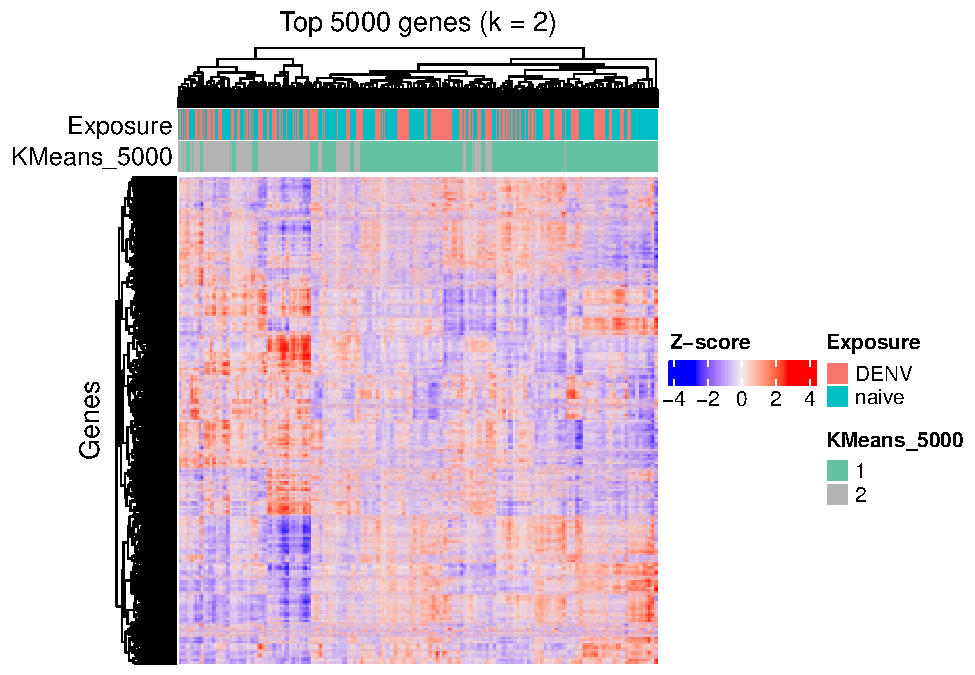
\includegraphics[keepaspectratio]{Assignment3_files/figure-latex/unnamed-chunk-5-1.pdf}}

\textbf{Metrics Table} I compared k-means fits for k = 2-8 across five
gene sets and recorded the average silhouette plus within-cluster
variation for each run. Every subset selected k = 2 with the highest
silhouette, reinforcing that a two-cluster solution best separates the
samples in a way consistent with the dengue-versus-naïve hypothesis.

\textbf{Chi-squared Table} I cross-tabulated each clustering (including
the k = 2 model on 5,000 genes) against exposure labels and against the
other gene-set clusterings, applying Benjamini-Hochberg correction. The
modest p-value for the 5,000-gene comparison shows partial alignment
with exposure status, while the extremely small p-values across gene-set
pairs confirm that different feature counts still yield highly
concordant cluster assignments.

\textbf{Heatmap} I visualized the scaled expression of the 5,000 genes
alongside exposure and k-means (k = 2) annotations. The two cluster bars
align with the heatmap's column dendrogram, letting us see how the major
expression split corresponds to the exposure groups reported in the
metadata.

\subsection{Ibrahim Zbib: Spectral
Clustering}\label{ibrahim-zbib-spectral-clustering}

\begin{Shaded}
\begin{Highlighting}[]
\FunctionTok{suppressPackageStartupMessages}\NormalTok{(\{}
  \FunctionTok{library}\NormalTok{(ggplot2)}
  \FunctionTok{library}\NormalTok{(grid)}
  \FunctionTok{library}\NormalTok{(glue)}
\NormalTok{\})}
\FunctionTok{suppressPackageStartupMessages}\NormalTok{(\{}
  \FunctionTok{library}\NormalTok{(purrr)}
  \FunctionTok{library}\NormalTok{(dplyr)}
  \FunctionTok{library}\NormalTok{(tibble)}
\NormalTok{\})}

\NormalTok{plots\_dir }\OtherTok{\textless{}{-}} \StringTok{"plots"}
\NormalTok{results\_dir }\OtherTok{\textless{}{-}} \StringTok{"results"}
\FunctionTok{dir.create}\NormalTok{(plots\_dir, }\AttributeTok{showWarnings =} \ConstantTok{FALSE}\NormalTok{, }\AttributeTok{recursive =} \ConstantTok{TRUE}\NormalTok{)}
\FunctionTok{dir.create}\NormalTok{(results\_dir, }\AttributeTok{showWarnings =} \ConstantTok{FALSE}\NormalTok{, }\AttributeTok{recursive =} \ConstantTok{TRUE}\NormalTok{)}

\NormalTok{save\_table\_png }\OtherTok{\textless{}{-}} \ControlFlowTok{function}\NormalTok{(df, path, }\AttributeTok{base\_height =} \DecValTok{400}\NormalTok{, }\AttributeTok{row\_px =} \DecValTok{28}\NormalTok{, }\AttributeTok{min\_width =} \DecValTok{1200}\NormalTok{)\{}
\NormalTok{  h }\OtherTok{\textless{}{-}} \FunctionTok{max}\NormalTok{(base\_height, }\FunctionTok{nrow}\NormalTok{(df) }\SpecialCharTok{*}\NormalTok{ row\_px }\SpecialCharTok{+} \DecValTok{120}\NormalTok{)}
\NormalTok{  w }\OtherTok{\textless{}{-}}\NormalTok{ min\_width}
\NormalTok{  g }\OtherTok{\textless{}{-}}\NormalTok{ gridExtra}\SpecialCharTok{::}\FunctionTok{tableGrob}\NormalTok{(df)}
  \FunctionTok{png}\NormalTok{(path, }\AttributeTok{width =}\NormalTok{ w, }\AttributeTok{height =}\NormalTok{ h, }\AttributeTok{res =} \DecValTok{150}\NormalTok{)}
\NormalTok{  grid}\SpecialCharTok{::}\FunctionTok{grid.newpage}\NormalTok{()}
\NormalTok{  grid}\SpecialCharTok{::}\FunctionTok{grid.draw}\NormalTok{(g)}
  \FunctionTok{dev.off}\NormalTok{()}
\NormalTok{\}}

\NormalTok{save\_gg\_png }\OtherTok{\textless{}{-}} \ControlFlowTok{function}\NormalTok{(plot, path, }\AttributeTok{width =} \DecValTok{10}\NormalTok{, }\AttributeTok{height =} \DecValTok{7}\NormalTok{, }\AttributeTok{dpi =} \DecValTok{300}\NormalTok{)\{}
\NormalTok{  ggplot2}\SpecialCharTok{::}\FunctionTok{ggsave}\NormalTok{(}\AttributeTok{filename =}\NormalTok{ path, }\AttributeTok{plot =}\NormalTok{ plot, }\AttributeTok{width =}\NormalTok{ width, }\AttributeTok{height =}\NormalTok{ height, }\AttributeTok{dpi =}\NormalTok{ dpi, }\AttributeTok{limitsize =} \ConstantTok{FALSE}\NormalTok{)}
\NormalTok{\}}
\end{Highlighting}
\end{Shaded}

\begin{Shaded}
\begin{Highlighting}[]
\ControlFlowTok{if}\NormalTok{ (}\SpecialCharTok{!}\FunctionTok{requireNamespace}\NormalTok{(}\StringTok{"kernlab"}\NormalTok{, }\AttributeTok{quietly =} \ConstantTok{TRUE}\NormalTok{)) \{}
  \FunctionTok{install.packages}\NormalTok{(}\StringTok{"kernlab"}\NormalTok{)}
\NormalTok{\}}
\FunctionTok{library}\NormalTok{(kernlab)}
\end{Highlighting}
\end{Shaded}

\begin{verbatim}
## Warning: package 'kernlab' was built under R version 4.5.2
\end{verbatim}

\begin{verbatim}
## 
## Attaching package: 'kernlab'
\end{verbatim}

\begin{verbatim}
## The following object is masked from 'package:scales':
## 
##     alpha
\end{verbatim}

\begin{verbatim}
## The following object is masked from 'package:purrr':
## 
##     cross
\end{verbatim}

\begin{verbatim}
## The following object is masked from 'package:BiocGenerics':
## 
##     type
\end{verbatim}

\begin{verbatim}
## The following object is masked from 'package:ggplot2':
## 
##     alpha
\end{verbatim}

\begin{Shaded}
\begin{Highlighting}[]
\FunctionTok{stopifnot}\NormalTok{(}\FunctionTok{exists}\NormalTok{(}\StringTok{"expression\_mat"}\NormalTok{), }\FunctionTok{exists}\NormalTok{(}\StringTok{"metadata"}\NormalTok{), }\FunctionTok{exists}\NormalTok{(}\StringTok{"expression\_top5000"}\NormalTok{))}


  
  \CommentTok{\#exposure\_lookup \textless{}{-} metadata\_exposure \%\textgreater{}\%}
   \CommentTok{\# select(refinebio\_accession\_code, Exposure) \%\textgreater{}\%}
    \CommentTok{\#mutate(Exposure = as.character(Exposure)) \%\textgreater{}\%}
    \CommentTok{\#deframe()}
  
\CommentTok{\#  exposure\_table \textless{}{-} metadata\_exposure \%\textgreater{}\%}
 \CommentTok{\#   transmute(}
  \CommentTok{\#    sample\_id = refinebio\_accession\_code,}
   \CommentTok{\#   exposure = as.character(Exposure)}
    \CommentTok{\#)}


\CommentTok{\# helper function to select top variable genes}
\NormalTok{select\_top\_genes }\OtherTok{\textless{}{-}} \ControlFlowTok{function}\NormalTok{(mat, n) \{}
\NormalTok{  n }\OtherTok{\textless{}{-}} \FunctionTok{min}\NormalTok{(n, }\FunctionTok{nrow}\NormalTok{(mat))}
\NormalTok{  variances }\OtherTok{\textless{}{-}}\NormalTok{ matrixStats}\SpecialCharTok{::}\FunctionTok{rowVars}\NormalTok{(mat)}
\NormalTok{  ordered }\OtherTok{\textless{}{-}} \FunctionTok{order}\NormalTok{(variances, }\AttributeTok{decreasing =} \ConstantTok{TRUE}\NormalTok{)}
\NormalTok{  idx }\OtherTok{\textless{}{-}} \FunctionTok{head}\NormalTok{(ordered, n)}
  \FunctionTok{list}\NormalTok{(}\AttributeTok{idx =}\NormalTok{ idx, }\AttributeTok{genes =} \FunctionTok{rownames}\NormalTok{(mat)[idx], }\AttributeTok{variances =}\NormalTok{ variances[idx])}
\NormalTok{\}}
\end{Highlighting}
\end{Shaded}

\subsubsection{2b-d: Running Spectral Clustering on 5000
genes}\label{b-d-running-spectral-clustering-on-5000-genes}

\begin{Shaded}
\begin{Highlighting}[]
\FunctionTok{cat}\NormalTok{(}\StringTok{"Running spectral clustering on 5000 most variable genes...}\SpecialCharTok{\textbackslash{}n\textbackslash{}n}\StringTok{"}\NormalTok{)}
\end{Highlighting}
\end{Shaded}

\begin{verbatim}
## Running spectral clustering on 5000 most variable genes...
\end{verbatim}

\begin{Shaded}
\begin{Highlighting}[]
\CommentTok{\# Use the expression\_top5000 matrix created in Section 2a}
\NormalTok{X\_5000 }\OtherTok{\textless{}{-}} \FunctionTok{t}\NormalTok{(expression\_top5000)}
\NormalTok{X\_5000\_scaled }\OtherTok{\textless{}{-}} \FunctionTok{scale}\NormalTok{(X\_5000)}
\NormalTok{X\_5000\_scaled[}\FunctionTok{is.na}\NormalTok{(X\_5000\_scaled)] }\OtherTok{\textless{}{-}} \DecValTok{0}

\NormalTok{k\_values }\OtherTok{\textless{}{-}} \DecValTok{2}\SpecialCharTok{:}\DecValTok{8}
\NormalTok{spectral\_results\_5000 }\OtherTok{\textless{}{-}} \FunctionTok{list}\NormalTok{()}

\ControlFlowTok{for}\NormalTok{ (k }\ControlFlowTok{in}\NormalTok{ k\_values) \{}
  \FunctionTok{cat}\NormalTok{(}\FunctionTok{glue}\NormalTok{(}\StringTok{"  Testing k = \{k\}...}\SpecialCharTok{\textbackslash{}n}\StringTok{"}\NormalTok{))}
  
\NormalTok{  sc\_fit }\OtherTok{\textless{}{-}} \FunctionTok{specc}\NormalTok{(X\_5000\_scaled, }\AttributeTok{centers =}\NormalTok{ k)}
  
  \CommentTok{\# Extract cluster assignments}
\NormalTok{  clusters }\OtherTok{\textless{}{-}} \FunctionTok{factor}\NormalTok{(sc\_fit}\SpecialCharTok{@}\NormalTok{.Data, }\AttributeTok{levels =} \FunctionTok{seq\_len}\NormalTok{(k))}
  \FunctionTok{names}\NormalTok{(clusters) }\OtherTok{\textless{}{-}} \FunctionTok{rownames}\NormalTok{(X\_5000\_scaled)}
  
  \CommentTok{\# silhouette for this k}
\NormalTok{  dist\_mat }\OtherTok{\textless{}{-}} \FunctionTok{dist}\NormalTok{(X\_5000\_scaled)}
\NormalTok{  sil }\OtherTok{\textless{}{-}} \FunctionTok{silhouette}\NormalTok{(}\FunctionTok{as.integer}\NormalTok{(clusters), dist\_mat)}
\NormalTok{  avg\_sil }\OtherTok{\textless{}{-}} \FunctionTok{mean}\NormalTok{(sil[, }\DecValTok{3}\NormalTok{])}
  
\NormalTok{  spectral\_results\_5000[[}\FunctionTok{as.character}\NormalTok{(k)]] }\OtherTok{\textless{}{-}} \FunctionTok{list}\NormalTok{(}
    \AttributeTok{k =}\NormalTok{ k,}
    \AttributeTok{clusters =}\NormalTok{ clusters,}
    \AttributeTok{avg\_silhouette =}\NormalTok{ avg\_sil,}
    \AttributeTok{silhouette\_obj =}\NormalTok{ sil}
\NormalTok{  )}
  
  \FunctionTok{cat}\NormalTok{(}\FunctionTok{glue}\NormalTok{(}\StringTok{"    Average silhouette: \{round(avg\_sil, 4)\}}\SpecialCharTok{\textbackslash{}n\textbackslash{}n}\StringTok{"}\NormalTok{))}
\NormalTok{\}}
\end{Highlighting}
\end{Shaded}

\begin{verbatim}
## Testing k = 2...Average silhouette: 0.3478
## Testing k = 3...Average silhouette: 0.0894
## Testing k = 4...Average silhouette: 0.0673
## Testing k = 5...Average silhouette: 0.068
## Testing k = 6...Average silhouette: 0.0459
## Testing k = 7...Average silhouette: 0.03
## Testing k = 8...Average silhouette: 0.0366
\end{verbatim}

\begin{Shaded}
\begin{Highlighting}[]
\NormalTok{k\_comparison\_5000 }\OtherTok{\textless{}{-}} \FunctionTok{map\_dfr}\NormalTok{(spectral\_results\_5000, }\ControlFlowTok{function}\NormalTok{(res) \{}
  \FunctionTok{tibble}\NormalTok{(}
    \AttributeTok{k =}\NormalTok{ res}\SpecialCharTok{$}\NormalTok{k,}
    \AttributeTok{avg\_silhouette =}\NormalTok{ res}\SpecialCharTok{$}\NormalTok{avg\_silhouette}
\NormalTok{  )}
\NormalTok{\})}
\end{Highlighting}
\end{Shaded}

\begin{Shaded}
\begin{Highlighting}[]
\FunctionTok{cat}\NormalTok{(}\StringTok{"}\SpecialCharTok{\textbackslash{}n}\StringTok{{-}{-}{-} How changing k affects results (5000 genes) {-}{-}{-}}\SpecialCharTok{\textbackslash{}n}\StringTok{"}\NormalTok{)}
\end{Highlighting}
\end{Shaded}

\begin{verbatim}
## 
## --- How changing k affects results (5000 genes) ---
\end{verbatim}

\begin{Shaded}
\begin{Highlighting}[]
\FunctionTok{print}\NormalTok{(k\_comparison\_5000)}
\end{Highlighting}
\end{Shaded}

\begin{verbatim}
## # A tibble: 7 x 2
##       k avg_silhouette
##   <int>          <dbl>
## 1     2         0.348 
## 2     3         0.0894
## 3     4         0.0673
## 4     5         0.0680
## 5     6         0.0459
## 6     7         0.0300
## 7     8         0.0366
\end{verbatim}

\begin{Shaded}
\begin{Highlighting}[]
\CommentTok{\# robust: base indexing; no dplyr::slice}
\NormalTok{best\_k\_5000 }\OtherTok{\textless{}{-}}\NormalTok{ k\_comparison\_5000}\SpecialCharTok{$}\NormalTok{k[}\FunctionTok{which.max}\NormalTok{(k\_comparison\_5000}\SpecialCharTok{$}\NormalTok{avg\_silhouette)]}

\FunctionTok{cat}\NormalTok{(}\FunctionTok{glue}\NormalTok{(}\StringTok{"}\SpecialCharTok{\textbackslash{}n}\StringTok{Best k selected: \{best\_k\_5000\} (highest silhouette score)}\SpecialCharTok{\textbackslash{}n\textbackslash{}n}\StringTok{"}\NormalTok{))}
\end{Highlighting}
\end{Shaded}

\begin{verbatim}
## Best k selected: 2 (highest silhouette score)
\end{verbatim}

\begin{Shaded}
\begin{Highlighting}[]
\NormalTok{spectral\_clusters\_5000\_best }\OtherTok{\textless{}{-}}\NormalTok{ spectral\_results\_5000[[}\FunctionTok{as.character}\NormalTok{(best\_k\_5000)]]}\SpecialCharTok{$}\NormalTok{clusters}

\FunctionTok{cat}\NormalTok{(}\StringTok{"{-}{-}{-} Comparing cluster membership across different k values {-}{-}{-}}\SpecialCharTok{\textbackslash{}n}\StringTok{"}\NormalTok{)}
\end{Highlighting}
\end{Shaded}

\begin{verbatim}
## --- Comparing cluster membership across different k values ---
\end{verbatim}

\begin{Shaded}
\begin{Highlighting}[]
\NormalTok{k\_pairs }\OtherTok{\textless{}{-}} \FunctionTok{combn}\NormalTok{(k\_values, }\DecValTok{2}\NormalTok{, }\AttributeTok{simplify =} \ConstantTok{FALSE}\NormalTok{)}

\NormalTok{chi\_sq\_k\_comparison }\OtherTok{\textless{}{-}} \FunctionTok{map\_dfr}\NormalTok{(k\_pairs, }\ControlFlowTok{function}\NormalTok{(pair) \{}
\NormalTok{  k1 }\OtherTok{\textless{}{-}}\NormalTok{ pair[}\DecValTok{1}\NormalTok{]}
\NormalTok{  k2 }\OtherTok{\textless{}{-}}\NormalTok{ pair[}\DecValTok{2}\NormalTok{]}
  
\NormalTok{  clust1 }\OtherTok{\textless{}{-}}\NormalTok{ spectral\_results\_5000[[}\FunctionTok{as.character}\NormalTok{(k1)]]}\SpecialCharTok{$}\NormalTok{clusters}
\NormalTok{  clust2 }\OtherTok{\textless{}{-}}\NormalTok{ spectral\_results\_5000[[}\FunctionTok{as.character}\NormalTok{(k2)]]}\SpecialCharTok{$}\NormalTok{clusters}
  
\NormalTok{  samples }\OtherTok{\textless{}{-}} \FunctionTok{intersect}\NormalTok{(}\FunctionTok{names}\NormalTok{(clust1), }\FunctionTok{names}\NormalTok{(clust2))}
\NormalTok{  clust1 }\OtherTok{\textless{}{-}}\NormalTok{ clust1[samples]}
\NormalTok{  clust2 }\OtherTok{\textless{}{-}}\NormalTok{ clust2[samples]}
  
\NormalTok{  tab }\OtherTok{\textless{}{-}} \FunctionTok{table}\NormalTok{(}\AttributeTok{k1 =}\NormalTok{ clust1, }\AttributeTok{k2 =}\NormalTok{ clust2)}
\NormalTok{  test }\OtherTok{\textless{}{-}} \FunctionTok{suppressWarnings}\NormalTok{(}\FunctionTok{chisq.test}\NormalTok{(tab))}
  
  \FunctionTok{tibble}\NormalTok{(}
    \AttributeTok{k1 =}\NormalTok{ k1,}
    \AttributeTok{k2 =}\NormalTok{ k2,}
    \AttributeTok{chi\_sq\_statistic =} \FunctionTok{unname}\NormalTok{(test}\SpecialCharTok{$}\NormalTok{statistic),}
    \AttributeTok{df =} \FunctionTok{unname}\NormalTok{(test}\SpecialCharTok{$}\NormalTok{parameter),}
    \AttributeTok{p\_value =}\NormalTok{ test}\SpecialCharTok{$}\NormalTok{p.value}
\NormalTok{  )}
\NormalTok{\})}
\end{Highlighting}
\end{Shaded}

\subsubsection{2e: Rerun clustering with different numbers of
genes}\label{e-rerun-clustering-with-different-numbers-of-genes}

\begin{Shaded}
\begin{Highlighting}[]
\FunctionTok{cat}\NormalTok{(}\StringTok{"}\SpecialCharTok{\textbackslash{}n\textbackslash{}n}\StringTok{=== Running spectral clustering on different gene counts ===}\SpecialCharTok{\textbackslash{}n\textbackslash{}n}\StringTok{"}\NormalTok{)}
\end{Highlighting}
\end{Shaded}

\begin{verbatim}
## 
## 
## === Running spectral clustering on different gene counts ===
\end{verbatim}

\begin{Shaded}
\begin{Highlighting}[]
\NormalTok{gene\_counts }\OtherTok{\textless{}{-}} \FunctionTok{c}\NormalTok{(}\DecValTok{10}\NormalTok{, }\DecValTok{100}\NormalTok{, }\DecValTok{1000}\NormalTok{, }\DecValTok{10000}\NormalTok{)}
\NormalTok{spectral\_all\_genes }\OtherTok{\textless{}{-}} \FunctionTok{list}\NormalTok{()}

\ControlFlowTok{for}\NormalTok{ (gene\_n }\ControlFlowTok{in}\NormalTok{ gene\_counts) \{}
  \FunctionTok{cat}\NormalTok{(}\FunctionTok{glue}\NormalTok{(}\StringTok{"{-}{-}{-} Processing \{gene\_n\} genes {-}{-}{-}}\SpecialCharTok{\textbackslash{}n}\StringTok{"}\NormalTok{))}
  
\NormalTok{  top }\OtherTok{\textless{}{-}} \FunctionTok{select\_top\_genes}\NormalTok{(expression\_mat, gene\_n)}
\NormalTok{  gene\_mat }\OtherTok{\textless{}{-}}\NormalTok{ expression\_mat[top}\SpecialCharTok{$}\NormalTok{idx, , drop }\OtherTok{=} \ConstantTok{FALSE}\NormalTok{]}
  
\NormalTok{  X }\OtherTok{\textless{}{-}} \FunctionTok{t}\NormalTok{(gene\_mat)}
\NormalTok{  X\_scaled }\OtherTok{\textless{}{-}} \FunctionTok{scale}\NormalTok{(X)}
\NormalTok{  X\_scaled[}\FunctionTok{is.na}\NormalTok{(X\_scaled)] }\OtherTok{\textless{}{-}} \DecValTok{0}
  
\NormalTok{  results\_this\_gene }\OtherTok{\textless{}{-}} \FunctionTok{list}\NormalTok{()}
  
  \ControlFlowTok{for}\NormalTok{ (k }\ControlFlowTok{in}\NormalTok{ k\_values) \{}
\NormalTok{    sc\_fit }\OtherTok{\textless{}{-}} \FunctionTok{specc}\NormalTok{(X\_scaled, }\AttributeTok{centers =}\NormalTok{ k)}
\NormalTok{    clusters }\OtherTok{\textless{}{-}} \FunctionTok{factor}\NormalTok{(sc\_fit}\SpecialCharTok{@}\NormalTok{.Data, }\AttributeTok{levels =} \FunctionTok{seq\_len}\NormalTok{(k))}
    \FunctionTok{names}\NormalTok{(clusters) }\OtherTok{\textless{}{-}} \FunctionTok{rownames}\NormalTok{(X\_scaled)}
    
\NormalTok{    dist\_mat }\OtherTok{\textless{}{-}} \FunctionTok{dist}\NormalTok{(X\_scaled)}
\NormalTok{    sil }\OtherTok{\textless{}{-}} \FunctionTok{silhouette}\NormalTok{(}\FunctionTok{as.integer}\NormalTok{(clusters), dist\_mat)}
\NormalTok{    avg\_sil }\OtherTok{\textless{}{-}} \FunctionTok{mean}\NormalTok{(sil[, }\DecValTok{3}\NormalTok{])}
    
\NormalTok{    results\_this\_gene[[}\FunctionTok{as.character}\NormalTok{(k)]] }\OtherTok{\textless{}{-}} \FunctionTok{list}\NormalTok{(}
      \AttributeTok{k =}\NormalTok{ k,}
      \AttributeTok{clusters =}\NormalTok{ clusters,}
      \AttributeTok{avg\_silhouette =}\NormalTok{ avg\_sil}
\NormalTok{    )}
\NormalTok{  \}}
  
\NormalTok{ best\_df }\OtherTok{\textless{}{-}} \FunctionTok{map\_dfr}\NormalTok{(results\_this\_gene, }\SpecialCharTok{\textasciitilde{}}\FunctionTok{tibble}\NormalTok{(}\AttributeTok{k =}\NormalTok{ .x}\SpecialCharTok{$}\NormalTok{k, }\AttributeTok{avg\_sil =}\NormalTok{ .x}\SpecialCharTok{$}\NormalTok{avg\_silhouette))}
\NormalTok{best\_k  }\OtherTok{\textless{}{-}}\NormalTok{ best\_df}\SpecialCharTok{$}\NormalTok{k[}\FunctionTok{which.max}\NormalTok{(best\_df}\SpecialCharTok{$}\NormalTok{avg\_sil)]}
  
  \FunctionTok{cat}\NormalTok{(}\FunctionTok{glue}\NormalTok{(}\StringTok{"  Best k = \{best\_k\} (silhouette = \{round(results\_this\_gene[[as.character(best\_k)]]$avg\_silhouette, 4)\})}\SpecialCharTok{\textbackslash{}n\textbackslash{}n}\StringTok{"}\NormalTok{))}
  
\NormalTok{  spectral\_all\_genes[[}\FunctionTok{paste0}\NormalTok{(}\StringTok{"genes\_"}\NormalTok{, gene\_n)]] }\OtherTok{\textless{}{-}} \FunctionTok{list}\NormalTok{(}
    \AttributeTok{gene\_count =}\NormalTok{ gene\_n,}
    \AttributeTok{results =}\NormalTok{ results\_this\_gene,}
    \AttributeTok{best\_k =}\NormalTok{ best\_k,}
    \AttributeTok{best\_clusters =}\NormalTok{ results\_this\_gene[[}\FunctionTok{as.character}\NormalTok{(best\_k)]]}\SpecialCharTok{$}\NormalTok{clusters}
\NormalTok{  )}
  
  \FunctionTok{gc}\NormalTok{()}
\NormalTok{\}}
\end{Highlighting}
\end{Shaded}

\begin{verbatim}
## --- Processing 10 genes ---Best k = 2 (silhouette = 0.2338)
## --- Processing 100 genes ---Best k = 6 (silhouette = 0.1434)
## --- Processing 1000 genes ---Best k = 2 (silhouette = 0.3721)
## --- Processing 10000 genes ---Best k = 2 (silhouette = 0.0937)
\end{verbatim}

\begin{Shaded}
\begin{Highlighting}[]
\NormalTok{spectral\_all\_genes[[}\StringTok{"genes\_5000"}\NormalTok{]] }\OtherTok{\textless{}{-}} \FunctionTok{list}\NormalTok{(}
  \AttributeTok{gene\_count =} \DecValTok{5000}\NormalTok{,}
  \AttributeTok{results =}\NormalTok{ spectral\_results\_5000,}
  \AttributeTok{best\_k =}\NormalTok{ best\_k\_5000,}
  \AttributeTok{best\_clusters =}\NormalTok{ spectral\_clusters\_5000\_best}
\NormalTok{)}

\NormalTok{best\_k\_summary }\OtherTok{\textless{}{-}} \FunctionTok{map\_dfr}\NormalTok{(spectral\_all\_genes, }\ControlFlowTok{function}\NormalTok{(x) \{}
  \FunctionTok{tibble}\NormalTok{(}
    \AttributeTok{gene\_count =}\NormalTok{ x}\SpecialCharTok{$}\NormalTok{gene\_count,}
    \AttributeTok{best\_k =}\NormalTok{ x}\SpecialCharTok{$}\NormalTok{best\_k,}
    \AttributeTok{avg\_silhouette =}\NormalTok{ x}\SpecialCharTok{$}\NormalTok{results[[}\FunctionTok{as.character}\NormalTok{(x}\SpecialCharTok{$}\NormalTok{best\_k)]]}\SpecialCharTok{$}\NormalTok{avg\_silhouette}
\NormalTok{  )}
\NormalTok{\}) }\SpecialCharTok{\%\textgreater{}\%} \FunctionTok{arrange}\NormalTok{(gene\_count)}

\FunctionTok{cat}\NormalTok{(}\StringTok{"}\SpecialCharTok{\textbackslash{}n}\StringTok{{-}{-}{-} Summary: Best k for each gene count {-}{-}{-}}\SpecialCharTok{\textbackslash{}n}\StringTok{"}\NormalTok{)}
\end{Highlighting}
\end{Shaded}

\begin{verbatim}
## 
## --- Summary: Best k for each gene count ---
\end{verbatim}

\begin{Shaded}
\begin{Highlighting}[]
\FunctionTok{print}\NormalTok{(best\_k\_summary)}
\end{Highlighting}
\end{Shaded}

\begin{verbatim}
## # A tibble: 5 x 3
##   gene_count best_k avg_silhouette
##        <dbl>  <int>          <dbl>
## 1         10      2         0.234 
## 2        100      6         0.143 
## 3       1000      2         0.372 
## 4       5000      2         0.348 
## 5      10000      2         0.0937
\end{verbatim}

\subsubsection{2e-i,ii: Chi-squared tests comparing clustering
results}\label{e-iii-chi-squared-tests-comparing-clustering-results}

\begin{Shaded}
\begin{Highlighting}[]
\FunctionTok{cat}\NormalTok{(}\StringTok{"}\SpecialCharTok{\textbackslash{}n\textbackslash{}n}\StringTok{=== Chi{-}squared tests comparing clustering results ===}\SpecialCharTok{\textbackslash{}n\textbackslash{}n}\StringTok{"}\NormalTok{)}
\end{Highlighting}
\end{Shaded}

\begin{verbatim}
## 
## 
## === Chi-squared tests comparing clustering results ===
\end{verbatim}

\begin{Shaded}
\begin{Highlighting}[]
\NormalTok{spectral\_best\_assignments }\OtherTok{\textless{}{-}}\NormalTok{ purrr}\SpecialCharTok{::}\FunctionTok{map}\NormalTok{(spectral\_all\_genes, }\StringTok{"best\_clusters"}\NormalTok{)}

\FunctionTok{cat}\NormalTok{(}\StringTok{"{-}{-}{-} Pairwise comparisons between different gene counts {-}{-}{-}}\SpecialCharTok{\textbackslash{}n}\StringTok{"}\NormalTok{)}
\end{Highlighting}
\end{Shaded}

\begin{verbatim}
## --- Pairwise comparisons between different gene counts ---
\end{verbatim}

\begin{Shaded}
\begin{Highlighting}[]
\NormalTok{gene\_count\_names }\OtherTok{\textless{}{-}} \FunctionTok{names}\NormalTok{(spectral\_best\_assignments)}
\NormalTok{gene\_pairs }\OtherTok{\textless{}{-}} \FunctionTok{combn}\NormalTok{(gene\_count\_names, }\DecValTok{2}\NormalTok{, }\AttributeTok{simplify =} \ConstantTok{FALSE}\NormalTok{)}

\NormalTok{safe\_chisq }\OtherTok{\textless{}{-}} \ControlFlowTok{function}\NormalTok{(a, b) \{}
  \ControlFlowTok{if}\NormalTok{ (}\FunctionTok{length}\NormalTok{(a) }\SpecialCharTok{!=} \FunctionTok{length}\NormalTok{(b)) }\FunctionTok{return}\NormalTok{(}\FunctionTok{list}\NormalTok{(}\AttributeTok{ok=}\ConstantTok{FALSE}\NormalTok{, }\AttributeTok{reason=}\StringTok{"length\_mismatch"}\NormalTok{, }\AttributeTok{test=}\ConstantTok{NULL}\NormalTok{))}
  \ControlFlowTok{if}\NormalTok{ (}\FunctionTok{length}\NormalTok{(a) }\SpecialCharTok{\textless{}} \DecValTok{2}\DataTypeTok{L}\NormalTok{)       }\FunctionTok{return}\NormalTok{(}\FunctionTok{list}\NormalTok{(}\AttributeTok{ok=}\ConstantTok{FALSE}\NormalTok{, }\AttributeTok{reason=}\StringTok{"too\_few\_samples"}\NormalTok{, }\AttributeTok{test=}\ConstantTok{NULL}\NormalTok{))}
\NormalTok{  tab }\OtherTok{\textless{}{-}} \FunctionTok{table}\NormalTok{(a, b)}
  \ControlFlowTok{if}\NormalTok{ (}\FunctionTok{nrow}\NormalTok{(tab) }\SpecialCharTok{\textless{}} \DecValTok{2}\DataTypeTok{L} \SpecialCharTok{||} \FunctionTok{ncol}\NormalTok{(tab) }\SpecialCharTok{\textless{}} \DecValTok{2}\DataTypeTok{L}\NormalTok{)}
    \FunctionTok{return}\NormalTok{(}\FunctionTok{list}\NormalTok{(}\AttributeTok{ok=}\ConstantTok{FALSE}\NormalTok{, }\AttributeTok{reason=}\StringTok{"table\_not\_2x2"}\NormalTok{, }\AttributeTok{test=}\ConstantTok{NULL}\NormalTok{))}
  \FunctionTok{list}\NormalTok{(}\AttributeTok{ok=}\ConstantTok{TRUE}\NormalTok{, }\AttributeTok{reason=}\ConstantTok{NA\_character\_}\NormalTok{, }\AttributeTok{test=}\FunctionTok{suppressWarnings}\NormalTok{(}\FunctionTok{chisq.test}\NormalTok{(tab)))}
\NormalTok{\}}

\NormalTok{chi\_sq\_gene\_pairs }\OtherTok{\textless{}{-}}\NormalTok{ purrr}\SpecialCharTok{::}\FunctionTok{map\_dfr}\NormalTok{(gene\_pairs, }\ControlFlowTok{function}\NormalTok{(pair) \{}
\NormalTok{  name1 }\OtherTok{\textless{}{-}}\NormalTok{ pair[}\DecValTok{1}\NormalTok{]; name2 }\OtherTok{\textless{}{-}}\NormalTok{ pair[}\DecValTok{2}\NormalTok{]}
\NormalTok{  g1 }\OtherTok{\textless{}{-}}\NormalTok{ spectral\_all\_genes[[name1]]; g2 }\OtherTok{\textless{}{-}}\NormalTok{ spectral\_all\_genes[[name2]]}

\NormalTok{  clust1 }\OtherTok{\textless{}{-}}\NormalTok{ spectral\_best\_assignments[[name1]]}
\NormalTok{  clust2 }\OtherTok{\textless{}{-}}\NormalTok{ spectral\_best\_assignments[[name2]]}

  
\NormalTok{  samples }\OtherTok{\textless{}{-}} \FunctionTok{intersect}\NormalTok{(}\FunctionTok{names}\NormalTok{(clust1), }\FunctionTok{names}\NormalTok{(clust2))}
\NormalTok{  clust1 }\OtherTok{\textless{}{-}}\NormalTok{ clust1[samples]}
\NormalTok{  clust2 }\OtherTok{\textless{}{-}}\NormalTok{ clust2[samples]}

\NormalTok{  res }\OtherTok{\textless{}{-}} \FunctionTok{safe\_chisq}\NormalTok{(clust1, clust2)}

  \ControlFlowTok{if}\NormalTok{ (}\SpecialCharTok{!}\NormalTok{res}\SpecialCharTok{$}\NormalTok{ok) \{}
    \FunctionTok{message}\NormalTok{(}\FunctionTok{sprintf}\NormalTok{(}\StringTok{"[skip \%s vs \%s] \%s | n=\%d"}\NormalTok{, name1, name2, res}\SpecialCharTok{$}\NormalTok{reason, }\FunctionTok{length}\NormalTok{(samples)))}
    \FunctionTok{return}\NormalTok{(tibble}\SpecialCharTok{::}\FunctionTok{tibble}\NormalTok{(}
      \AttributeTok{comparison =} \StringTok{"gene\_counts"}\NormalTok{,}
      \AttributeTok{gene\_count\_a =}\NormalTok{ g1}\SpecialCharTok{$}\NormalTok{gene\_count,}
      \AttributeTok{gene\_count\_b =}\NormalTok{ g2}\SpecialCharTok{$}\NormalTok{gene\_count,}
      \AttributeTok{k\_a =}\NormalTok{ g1}\SpecialCharTok{$}\NormalTok{best\_k,}
      \AttributeTok{k\_b =}\NormalTok{ g2}\SpecialCharTok{$}\NormalTok{best\_k,}
      \AttributeTok{chi\_sq\_statistic =} \ConstantTok{NA\_real\_}\NormalTok{,}
      \AttributeTok{df =} \ConstantTok{NA\_real\_}\NormalTok{,}
      \AttributeTok{p\_value =} \ConstantTok{NA\_real\_}\NormalTok{,}
      \AttributeTok{note =}\NormalTok{ res}\SpecialCharTok{$}\NormalTok{reason}
\NormalTok{    ))}
\NormalTok{  \}}

\NormalTok{  tibble}\SpecialCharTok{::}\FunctionTok{tibble}\NormalTok{(}
    \AttributeTok{comparison =} \StringTok{"gene\_counts"}\NormalTok{,}
    \AttributeTok{gene\_count\_a =}\NormalTok{ g1}\SpecialCharTok{$}\NormalTok{gene\_count,}
    \AttributeTok{gene\_count\_b =}\NormalTok{ g2}\SpecialCharTok{$}\NormalTok{gene\_count,}
    \AttributeTok{k\_a =}\NormalTok{ g1}\SpecialCharTok{$}\NormalTok{best\_k,}
    \AttributeTok{k\_b =}\NormalTok{ g2}\SpecialCharTok{$}\NormalTok{best\_k,}
    \AttributeTok{chi\_sq\_statistic =} \FunctionTok{unname}\NormalTok{(res}\SpecialCharTok{$}\NormalTok{test}\SpecialCharTok{$}\NormalTok{statistic),}
    \AttributeTok{df =} \FunctionTok{unname}\NormalTok{(res}\SpecialCharTok{$}\NormalTok{test}\SpecialCharTok{$}\NormalTok{parameter),}
    \AttributeTok{p\_value =}\NormalTok{ res}\SpecialCharTok{$}\NormalTok{test}\SpecialCharTok{$}\NormalTok{p.value,}
    \AttributeTok{note =} \ConstantTok{NA\_character\_}
\NormalTok{  )}
\NormalTok{\})}

\FunctionTok{print}\NormalTok{(chi\_sq\_gene\_pairs)}
\end{Highlighting}
\end{Shaded}

\begin{verbatim}
## # A tibble: 10 x 9
##    comparison  gene_count_a gene_count_b   k_a   k_b chi_sq_statistic    df
##    <chr>              <dbl>        <dbl> <int> <int>            <dbl> <int>
##  1 gene_counts           10          100     2     6         3.35e+ 2     5
##  2 gene_counts           10         1000     2     2         1.99e-26     1
##  3 gene_counts           10        10000     2     2         1.56e+ 0     1
##  4 gene_counts           10         5000     2     2         1.99e-26     1
##  5 gene_counts          100         1000     6     2         7.83e+ 0     5
##  6 gene_counts          100        10000     6     2         3.28e+ 2     5
##  7 gene_counts          100         5000     6     2         7.83e+ 0     5
##  8 gene_counts         1000        10000     2     2         2.61e+ 0     1
##  9 gene_counts         1000         5000     2     2         5.74e+ 2     1
## 10 gene_counts        10000         5000     2     2         2.61e+ 0     1
## # i 2 more variables: p_value <dbl>, note <chr>
\end{verbatim}

\begin{Shaded}
\begin{Highlighting}[]
\FunctionTok{suppressPackageStartupMessages}\NormalTok{(\{}
  \FunctionTok{library}\NormalTok{(pheatmap)}
  \FunctionTok{library}\NormalTok{(RColorBrewer)}
  \FunctionTok{library}\NormalTok{(glue)}
\NormalTok{\})}
\end{Highlighting}
\end{Shaded}

\begin{verbatim}
## Warning: package 'pheatmap' was built under R version 4.5.2
\end{verbatim}

\begin{Shaded}
\begin{Highlighting}[]
\CommentTok{\# {-}{-}{-} data prep (same as before) {-}{-}{-}}
\NormalTok{heatmap\_matrix }\OtherTok{\textless{}{-}} \FunctionTok{log2}\NormalTok{(expression\_top5000 }\SpecialCharTok{+} \DecValTok{1}\NormalTok{)}
\NormalTok{heatmap\_matrix }\OtherTok{\textless{}{-}} \FunctionTok{t}\NormalTok{(}\FunctionTok{scale}\NormalTok{(}\FunctionTok{t}\NormalTok{(heatmap\_matrix)))}
\NormalTok{heatmap\_matrix[}\SpecialCharTok{!}\FunctionTok{is.finite}\NormalTok{(heatmap\_matrix)] }\OtherTok{\textless{}{-}} \DecValTok{0}
\NormalTok{heatmap\_samples }\OtherTok{\textless{}{-}} \FunctionTok{colnames}\NormalTok{(heatmap\_matrix)}

\CommentTok{\#align annotations}
\NormalTok{spectral\_col }\OtherTok{\textless{}{-}} \FunctionTok{as.character}\NormalTok{(spectral\_clusters\_5000\_best[heatmap\_samples])}
\NormalTok{exposure\_col }\OtherTok{\textless{}{-}} \FunctionTok{as.character}\NormalTok{(exposure\_lookup[heatmap\_samples])}
\NormalTok{exposure\_col[}\FunctionTok{is.na}\NormalTok{(exposure\_col)] }\OtherTok{\textless{}{-}} \StringTok{"Unknown"}

\CommentTok{\#factors AFTER alignment}
\NormalTok{spectral\_factor }\OtherTok{\textless{}{-}} \FunctionTok{factor}\NormalTok{(spectral\_col)}
\NormalTok{exposure\_factor }\OtherTok{\textless{}{-}} \FunctionTok{factor}\NormalTok{(exposure\_col)}

\CommentTok{\# annotation data frame }
\NormalTok{annotation\_col }\OtherTok{\textless{}{-}} \FunctionTok{data.frame}\NormalTok{(}
  \AttributeTok{Exposure =}\NormalTok{ exposure\_factor,}
  \AttributeTok{Spectral =}\NormalTok{ spectral\_factor,}
  \AttributeTok{row.names =}\NormalTok{ heatmap\_samples}
\NormalTok{)}

\CommentTok{\# annotation colors}
\NormalTok{mk\_cols }\OtherTok{\textless{}{-}} \ControlFlowTok{function}\NormalTok{(n, pal) \{}
  \FunctionTok{colorRampPalette}\NormalTok{(}\FunctionTok{brewer.pal}\NormalTok{(}\DecValTok{8}\NormalTok{, pal))(}\FunctionTok{max}\NormalTok{(}\DecValTok{1}\DataTypeTok{L}\NormalTok{, n))}
\NormalTok{\}}
\NormalTok{ann\_colors }\OtherTok{\textless{}{-}} \FunctionTok{list}\NormalTok{(}
  \AttributeTok{Exposure =} \FunctionTok{setNames}\NormalTok{(}\FunctionTok{mk\_cols}\NormalTok{(}\FunctionTok{nlevels}\NormalTok{(exposure\_factor), }\StringTok{"Dark2"}\NormalTok{), }\FunctionTok{levels}\NormalTok{(exposure\_factor)),}
  \AttributeTok{Spectral =} \FunctionTok{setNames}\NormalTok{(}\FunctionTok{mk\_cols}\NormalTok{(}\FunctionTok{nlevels}\NormalTok{(spectral\_factor), }\StringTok{"Set3"}\NormalTok{),  }\FunctionTok{levels}\NormalTok{(spectral\_factor))}
\NormalTok{)}

\CommentTok{\# heatmap colors }
\NormalTok{hm\_cols }\OtherTok{\textless{}{-}} \FunctionTok{colorRampPalette}\NormalTok{(}\FunctionTok{c}\NormalTok{(}\StringTok{"navy"}\NormalTok{, }\StringTok{"white"}\NormalTok{, }\StringTok{"firebrick3"}\NormalTok{))(}\DecValTok{101}\NormalTok{)}

\NormalTok{title\_text }\OtherTok{\textless{}{-}} \ControlFlowTok{if}\NormalTok{ (}\FunctionTok{exists}\NormalTok{(}\StringTok{"best\_k\_5000"}\NormalTok{) }\SpecialCharTok{\&\&} \SpecialCharTok{!}\FunctionTok{is.na}\NormalTok{(best\_k\_5000)) \{}
  \FunctionTok{glue}\NormalTok{(}\StringTok{"Top 5000 genes {-} Spectral (k = \{best\_k\_5000\})"}\NormalTok{)}
\NormalTok{\} }\ControlFlowTok{else} \StringTok{"Top 5000 genes {-} Spectral"}


\ControlFlowTok{if}\NormalTok{ (}\SpecialCharTok{!}\FunctionTok{exists}\NormalTok{(}\StringTok{"plots\_dir"}\NormalTok{)) plots\_dir }\OtherTok{\textless{}{-}} \StringTok{"plots"}
\ControlFlowTok{if}\NormalTok{ (}\SpecialCharTok{!}\FunctionTok{dir.exists}\NormalTok{(plots\_dir)) }\FunctionTok{dir.create}\NormalTok{(plots\_dir, }\AttributeTok{recursive =} \ConstantTok{TRUE}\NormalTok{)}

\FunctionTok{dir.create}\NormalTok{(}\StringTok{"plots"}\NormalTok{, }\AttributeTok{showWarnings =} \ConstantTok{FALSE}\NormalTok{, }\AttributeTok{recursive =} \ConstantTok{TRUE}\NormalTok{)}

\NormalTok{ph }\OtherTok{\textless{}{-}} \FunctionTok{pheatmap}\NormalTok{(}
  \AttributeTok{mat =}\NormalTok{ heatmap\_matrix,}
  \AttributeTok{color =}\NormalTok{ hm\_cols,}
  \AttributeTok{cluster\_rows =} \ConstantTok{TRUE}\NormalTok{,}
  \AttributeTok{cluster\_cols =} \ConstantTok{TRUE}\NormalTok{,}
  \AttributeTok{show\_rownames =} \ConstantTok{FALSE}\NormalTok{,}
  \AttributeTok{show\_colnames =} \ConstantTok{FALSE}\NormalTok{,}
  \AttributeTok{annotation\_col =}\NormalTok{ annotation\_col,}
  \AttributeTok{annotation\_colors =}\NormalTok{ ann\_colors,}
  \AttributeTok{main =}\NormalTok{ title\_text,}
  \AttributeTok{legend =} \ConstantTok{TRUE}\NormalTok{,}
  \AttributeTok{fontsize =} \DecValTok{10}\NormalTok{,}
  \AttributeTok{border\_color =} \ConstantTok{NA}\NormalTok{,}
  \AttributeTok{filename =} \FunctionTok{file.path}\NormalTok{(}\StringTok{"plots"}\NormalTok{, }\StringTok{"spectral\_heatmap\_top5000.png"}\NormalTok{)  }\CommentTok{\# writes to disk}
\NormalTok{)}

\FunctionTok{print}\NormalTok{(}\FunctionTok{normalizePath}\NormalTok{(}\FunctionTok{file.path}\NormalTok{(}\StringTok{"plots"}\NormalTok{, }\StringTok{"spectral\_heatmap\_top5000.png"}\NormalTok{), }\AttributeTok{winslash =} \StringTok{"/"}\NormalTok{))}
\end{Highlighting}
\end{Shaded}

\begin{verbatim}
## [1] "C:/Users/Taylo/OneDrive - University of Florida/Current Classes/Bioinformatics/BioinformaticsProject/plots/spectral_heatmap_top5000.png"
\end{verbatim}

\subsubsection{4a: Statistical comparison with Assignment 1
groups}\label{a-statistical-comparison-with-assignment-1-groups}

\begin{Shaded}
\begin{Highlighting}[]
\FunctionTok{cat}\NormalTok{(}\StringTok{"}\SpecialCharTok{\textbackslash{}n\textbackslash{}n}\StringTok{=== Comparing clusters with Assignment 1 groups ===}\SpecialCharTok{\textbackslash{}n\textbackslash{}n}\StringTok{"}\NormalTok{)}
\end{Highlighting}
\end{Shaded}

\begin{verbatim}
## 
## 
## === Comparing clusters with Assignment 1 groups ===
\end{verbatim}

\begin{Shaded}
\begin{Highlighting}[]
\NormalTok{chi\_sq\_vs\_assignment1 }\OtherTok{\textless{}{-}} \FunctionTok{map\_dfr}\NormalTok{(}\FunctionTok{names}\NormalTok{(spectral\_all\_genes), }\ControlFlowTok{function}\NormalTok{(name) \{}
\NormalTok{  gene\_n }\OtherTok{\textless{}{-}}\NormalTok{ spectral\_all\_genes[[name]]}\SpecialCharTok{$}\NormalTok{gene\_count}
\NormalTok{  best\_k }\OtherTok{\textless{}{-}}\NormalTok{ spectral\_all\_genes[[name]]}\SpecialCharTok{$}\NormalTok{best\_k}
\NormalTok{  clusters }\OtherTok{\textless{}{-}}\NormalTok{ spectral\_all\_genes[[name]]}\SpecialCharTok{$}\NormalTok{best\_clusters}
  
  
\NormalTok{  samples }\OtherTok{\textless{}{-}} \FunctionTok{names}\NormalTok{(clusters)}
\NormalTok{  exposures }\OtherTok{\textless{}{-}}\NormalTok{ exposure\_lookup[samples]}
\NormalTok{  exposures[}\FunctionTok{is.na}\NormalTok{(exposures)] }\OtherTok{\textless{}{-}} \StringTok{"Unknown"}
  
  
\NormalTok{  tab }\OtherTok{\textless{}{-}} \FunctionTok{table}\NormalTok{(}
    \AttributeTok{exposure =} \FunctionTok{factor}\NormalTok{(exposures),}
    \AttributeTok{cluster =}\NormalTok{ clusters}
\NormalTok{  )}
\NormalTok{  test }\OtherTok{\textless{}{-}} \FunctionTok{suppressWarnings}\NormalTok{(}\FunctionTok{chisq.test}\NormalTok{(tab))}
  
  \FunctionTok{tibble}\NormalTok{(}
    \AttributeTok{comparison =} \StringTok{"clusters\_vs\_assignment1"}\NormalTok{,}
    \AttributeTok{gene\_count =}\NormalTok{ gene\_n,}
    \AttributeTok{k =}\NormalTok{ best\_k,}
    \AttributeTok{chi\_sq\_statistic =} \FunctionTok{unname}\NormalTok{(test}\SpecialCharTok{$}\NormalTok{statistic),}
    \AttributeTok{df =} \FunctionTok{unname}\NormalTok{(test}\SpecialCharTok{$}\NormalTok{parameter),}
    \AttributeTok{p\_value =}\NormalTok{ test}\SpecialCharTok{$}\NormalTok{p.value}
\NormalTok{  )}
\NormalTok{\})}

\FunctionTok{cat}\NormalTok{(}\StringTok{"{-}{-}{-} Chi{-}squared tests: Spectral clusters vs Assignment 1 groups {-}{-}{-}}\SpecialCharTok{\textbackslash{}n}\StringTok{"}\NormalTok{)}
\end{Highlighting}
\end{Shaded}

\begin{verbatim}
## --- Chi-squared tests: Spectral clusters vs Assignment 1 groups ---
\end{verbatim}

\begin{Shaded}
\begin{Highlighting}[]
\FunctionTok{print}\NormalTok{(chi\_sq\_vs\_assignment1)}
\end{Highlighting}
\end{Shaded}

\begin{verbatim}
## # A tibble: 5 x 6
##   comparison              gene_count     k chi_sq_statistic    df  p_value
##   <chr>                        <dbl> <int>            <dbl> <int>    <dbl>
## 1 clusters_vs_assignment1         10     2            5.09      1 2.41e- 2
## 2 clusters_vs_assignment1        100     6           59.3       5 1.66e-11
## 3 clusters_vs_assignment1       1000     2            0.350     1 5.54e- 1
## 4 clusters_vs_assignment1      10000     2            4.55      1 3.29e- 2
## 5 clusters_vs_assignment1       5000     2            0.350     1 5.54e- 1
\end{verbatim}

\begin{Shaded}
\begin{Highlighting}[]
\NormalTok{readr}\SpecialCharTok{::}\FunctionTok{write\_tsv}\NormalTok{(k\_comparison\_5000, }\FunctionTok{file.path}\NormalTok{(results\_dir, }\StringTok{"spectral\_k\_comparison\_5000.tsv"}\NormalTok{))}
\FunctionTok{save\_table\_png}\NormalTok{(k\_comparison\_5000, }\FunctionTok{file.path}\NormalTok{(plots\_dir, }\StringTok{"spectral\_k\_comparison\_5000.png"}\NormalTok{))}
\end{Highlighting}
\end{Shaded}

\begin{verbatim}
## pdf 
##   2
\end{verbatim}

\begin{Shaded}
\begin{Highlighting}[]
\FunctionTok{save\_table\_png}\NormalTok{(chi\_sq\_k\_comparison, }\FunctionTok{file.path}\NormalTok{(plots\_dir, }\StringTok{"spectral\_chi\_sq\_k\_comparison\_5000.png"}\NormalTok{))}
\end{Highlighting}
\end{Shaded}

\begin{verbatim}
## pdf 
##   2
\end{verbatim}

\begin{Shaded}
\begin{Highlighting}[]
\FunctionTok{install.packages}\NormalTok{(}\StringTok{"gridExtra"}\NormalTok{)}
\end{Highlighting}
\end{Shaded}

\begin{verbatim}
## Installing package into 'C:/Users/Taylo/AppData/Local/R/win-library/4.5'
## (as 'lib' is unspecified)
\end{verbatim}

\begin{verbatim}
## package 'gridExtra' successfully unpacked and MD5 sums checked
## 
## The downloaded binary packages are in
##  C:\Users\Taylo\AppData\Local\Temp\RtmpM7ItbU\downloaded_packages
\end{verbatim}

\begin{Shaded}
\begin{Highlighting}[]
\FunctionTok{library}\NormalTok{(gridExtra); }\FunctionTok{library}\NormalTok{(grid)}
\end{Highlighting}
\end{Shaded}

\begin{verbatim}
## Warning: package 'gridExtra' was built under R version 4.5.2
\end{verbatim}

\begin{verbatim}
## 
## Attaching package: 'gridExtra'
\end{verbatim}

\begin{verbatim}
## The following object is masked from 'package:Biobase':
## 
##     combine
\end{verbatim}

\begin{verbatim}
## The following object is masked from 'package:BiocGenerics':
## 
##     combine
\end{verbatim}

\begin{verbatim}
## The following object is masked from 'package:dplyr':
## 
##     combine
\end{verbatim}

\begin{Shaded}
\begin{Highlighting}[]
\NormalTok{save\_table\_png }\OtherTok{\textless{}{-}} \ControlFlowTok{function}\NormalTok{(df, path, }\AttributeTok{base\_size =} \DecValTok{10}\NormalTok{, }\AttributeTok{dpi =} \DecValTok{200}\NormalTok{, }\AttributeTok{min\_w =} \DecValTok{8}\NormalTok{, }\AttributeTok{min\_h =} \DecValTok{4}\NormalTok{)\{}
\NormalTok{  tb }\OtherTok{\textless{}{-}} \FunctionTok{tableGrob}\NormalTok{(df, }\AttributeTok{rows =} \ConstantTok{NULL}\NormalTok{, }\AttributeTok{theme =} \FunctionTok{ttheme\_minimal}\NormalTok{(}\AttributeTok{base\_size =}\NormalTok{ base\_size))}
  \FunctionTok{png}\NormalTok{(}\FunctionTok{tempfile}\NormalTok{(}\AttributeTok{fileext =} \StringTok{".png"}\NormalTok{), }\AttributeTok{width =} \DecValTok{10}\NormalTok{, }\AttributeTok{height =} \DecValTok{10}\NormalTok{, }\AttributeTok{units =} \StringTok{"in"}\NormalTok{, }\AttributeTok{res =}\NormalTok{ dpi)}
  \FunctionTok{grid.newpage}\NormalTok{(); }\FunctionTok{grid.draw}\NormalTok{(tb)}
\NormalTok{  w\_in }\OtherTok{\textless{}{-}} \FunctionTok{convertWidth}\NormalTok{(}\FunctionTok{sum}\NormalTok{(tb}\SpecialCharTok{$}\NormalTok{widths), }\StringTok{"in"}\NormalTok{, }\AttributeTok{valueOnly =} \ConstantTok{TRUE}\NormalTok{)}
\NormalTok{  h\_in }\OtherTok{\textless{}{-}} \FunctionTok{convertHeight}\NormalTok{(}\FunctionTok{sum}\NormalTok{(tb}\SpecialCharTok{$}\NormalTok{heights), }\StringTok{"in"}\NormalTok{, }\AttributeTok{valueOnly =} \ConstantTok{TRUE}\NormalTok{)}
  \FunctionTok{dev.off}\NormalTok{()}
\NormalTok{  w }\OtherTok{\textless{}{-}} \FunctionTok{max}\NormalTok{(min\_w, w\_in); h }\OtherTok{\textless{}{-}} \FunctionTok{max}\NormalTok{(min\_h, h\_in)}
  \FunctionTok{png}\NormalTok{(path, }\AttributeTok{width =}\NormalTok{ w, }\AttributeTok{height =}\NormalTok{ h, }\AttributeTok{units =} \StringTok{"in"}\NormalTok{, }\AttributeTok{res =}\NormalTok{ dpi)}
  \FunctionTok{grid.newpage}\NormalTok{(); }\FunctionTok{grid.draw}\NormalTok{(tb)}
  \FunctionTok{dev.off}\NormalTok{()}
\NormalTok{\}}

\FunctionTok{save\_table\_png}\NormalTok{(k\_comparison\_5000, }\FunctionTok{file.path}\NormalTok{(}\StringTok{"plots"}\NormalTok{,}\StringTok{"spectral\_k\_comparison\_5000.png"}\NormalTok{))}
\end{Highlighting}
\end{Shaded}

\begin{verbatim}
## pdf 
##   2
\end{verbatim}

\begin{Shaded}
\begin{Highlighting}[]
\FunctionTok{save\_table\_png}\NormalTok{(chi\_sq\_k\_comparison, }\FunctionTok{file.path}\NormalTok{(}\StringTok{"plots"}\NormalTok{,}\StringTok{"spectral\_chi\_sq\_k\_comparison\_5000.png"}\NormalTok{))}
\end{Highlighting}
\end{Shaded}

\begin{verbatim}
## pdf 
##   2
\end{verbatim}

\begin{Shaded}
\begin{Highlighting}[]
\FunctionTok{save\_table\_png}\NormalTok{(best\_k\_summary, }\FunctionTok{file.path}\NormalTok{(}\StringTok{"plots"}\NormalTok{,}\StringTok{"spectral\_best\_k\_summary.png"}\NormalTok{))}
\end{Highlighting}
\end{Shaded}

\begin{verbatim}
## pdf 
##   2
\end{verbatim}

\begin{Shaded}
\begin{Highlighting}[]
\FunctionTok{save\_table\_png}\NormalTok{(chi\_sq\_gene\_pairs, }\FunctionTok{file.path}\NormalTok{(}\StringTok{"plots"}\NormalTok{,}\StringTok{"spectral\_chi\_sq\_gene\_pairs.png"}\NormalTok{))}
\end{Highlighting}
\end{Shaded}

\begin{verbatim}
## pdf 
##   2
\end{verbatim}

\begin{Shaded}
\begin{Highlighting}[]
\FunctionTok{save\_table\_png}\NormalTok{(chi\_sq\_vs\_assignment1, }\FunctionTok{file.path}\NormalTok{(}\StringTok{"plots"}\NormalTok{,}\StringTok{"spectral\_chi\_sq\_vs\_assignment1.png"}\NormalTok{))}
\end{Highlighting}
\end{Shaded}

\begin{verbatim}
## pdf 
##   2
\end{verbatim}

\subsubsection{4b: Adjust for multiple hypothesis
testing}\label{b-adjust-for-multiple-hypothesis-testing}

\begin{Shaded}
\begin{Highlighting}[]
\FunctionTok{cat}\NormalTok{(}\StringTok{"}\SpecialCharTok{\textbackslash{}n\textbackslash{}n}\StringTok{=== Adjusting p{-}values for multiple testing ===}\SpecialCharTok{\textbackslash{}n\textbackslash{}n}\StringTok{"}\NormalTok{)}
\end{Highlighting}
\end{Shaded}

\begin{verbatim}
## 
## 
## === Adjusting p-values for multiple testing ===
\end{verbatim}

\begin{Shaded}
\begin{Highlighting}[]
\FunctionTok{library}\NormalTok{(dplyr)}
\CommentTok{\#combine all chi{-}squared tests}
\NormalTok{all\_chi\_sq\_tests }\OtherTok{\textless{}{-}} \FunctionTok{bind\_rows}\NormalTok{(}
\NormalTok{  chi\_sq\_gene\_pairs,}
\NormalTok{  chi\_sq\_vs\_assignment1 }\SpecialCharTok{\%\textgreater{}\%} 
    \FunctionTok{transmute}\NormalTok{(}
\NormalTok{      comparison,}
      \AttributeTok{gene\_count\_a =}\NormalTok{ gene\_count,}
      \AttributeTok{gene\_count\_b =}\NormalTok{ gene\_count,}
      \AttributeTok{k\_a =}\NormalTok{ k,}
      \AttributeTok{k\_b =}\NormalTok{ k,}
\NormalTok{      chi\_sq\_statistic,}
\NormalTok{      df,}
\NormalTok{      p\_value}
\NormalTok{    )}
\NormalTok{) }\SpecialCharTok{\%\textgreater{}\%}
  \FunctionTok{mutate}\NormalTok{(}\AttributeTok{p\_adj\_BH =} \FunctionTok{p.adjust}\NormalTok{(p\_value, }\AttributeTok{method =} \StringTok{"BH"}\NormalTok{)) }\SpecialCharTok{\%\textgreater{}\%}
  \FunctionTok{arrange}\NormalTok{(comparison, gene\_count\_a, gene\_count\_b)}

\FunctionTok{cat}\NormalTok{(}\StringTok{"{-}{-}{-} All chi{-}squared tests with adjusted p{-}values {-}{-}{-}}\SpecialCharTok{\textbackslash{}n}\StringTok{"}\NormalTok{)}
\end{Highlighting}
\end{Shaded}

\begin{verbatim}
## --- All chi-squared tests with adjusted p-values ---
\end{verbatim}

\begin{Shaded}
\begin{Highlighting}[]
\FunctionTok{print}\NormalTok{(all\_chi\_sq\_tests)}
\end{Highlighting}
\end{Shaded}

\begin{verbatim}
## # A tibble: 15 x 10
##    comparison       gene_count_a gene_count_b   k_a   k_b chi_sq_statistic    df
##    <chr>                   <dbl>        <dbl> <int> <int>            <dbl> <int>
##  1 clusters_vs_ass~           10           10     2     2         5.09e+ 0     1
##  2 clusters_vs_ass~          100          100     6     6         5.93e+ 1     5
##  3 clusters_vs_ass~         1000         1000     2     2         3.50e- 1     1
##  4 clusters_vs_ass~         5000         5000     2     2         3.50e- 1     1
##  5 clusters_vs_ass~        10000        10000     2     2         4.55e+ 0     1
##  6 gene_counts                10          100     2     6         3.35e+ 2     5
##  7 gene_counts                10         1000     2     2         1.99e-26     1
##  8 gene_counts                10         5000     2     2         1.99e-26     1
##  9 gene_counts                10        10000     2     2         1.56e+ 0     1
## 10 gene_counts               100         1000     6     2         7.83e+ 0     5
## 11 gene_counts               100         5000     6     2         7.83e+ 0     5
## 12 gene_counts               100        10000     6     2         3.28e+ 2     5
## 13 gene_counts              1000         5000     2     2         5.74e+ 2     1
## 14 gene_counts              1000        10000     2     2         2.61e+ 0     1
## 15 gene_counts             10000         5000     2     2         2.61e+ 0     1
## # i 3 more variables: p_value <dbl>, note <chr>, p_adj_BH <dbl>
\end{verbatim}

\begin{Shaded}
\begin{Highlighting}[]
\ControlFlowTok{if}\NormalTok{ (}\SpecialCharTok{!}\FunctionTok{exists}\NormalTok{(}\StringTok{"results\_dir"}\NormalTok{)) \{}
\NormalTok{  results\_dir }\OtherTok{\textless{}{-}} \StringTok{"results"}
\NormalTok{\}}
\ControlFlowTok{if}\NormalTok{ (}\SpecialCharTok{!}\FunctionTok{dir.exists}\NormalTok{(results\_dir)) }\FunctionTok{dir.create}\NormalTok{(results\_dir, }\AttributeTok{recursive =} \ConstantTok{TRUE}\NormalTok{)}

\NormalTok{readr}\SpecialCharTok{::}\FunctionTok{write\_tsv}\NormalTok{(best\_k\_summary, }\FunctionTok{file.path}\NormalTok{(results\_dir, }\StringTok{"spectral\_best\_k\_summary.tsv"}\NormalTok{))}
\NormalTok{readr}\SpecialCharTok{::}\FunctionTok{write\_tsv}\NormalTok{(all\_chi\_sq\_tests, }\FunctionTok{file.path}\NormalTok{(results\_dir, }\StringTok{"spectral\_chisq\_tests.tsv"}\NormalTok{))}
\NormalTok{readr}\SpecialCharTok{::}\FunctionTok{write\_tsv}\NormalTok{(k\_comparison\_5000, }\FunctionTok{file.path}\NormalTok{(results\_dir, }\StringTok{"spectral\_k\_comparison\_5000genes.tsv"}\NormalTok{))}

\FunctionTok{save\_table\_png}\NormalTok{(all\_chi\_sq\_tests, }\FunctionTok{file.path}\NormalTok{(}\StringTok{"plots"}\NormalTok{,}\StringTok{"spectral\_all\_chi\_sq\_tests.png"}\NormalTok{))}
\end{Highlighting}
\end{Shaded}

\begin{verbatim}
## pdf 
##   2
\end{verbatim}

\begin{Shaded}
\begin{Highlighting}[]
\FunctionTok{assign}\NormalTok{(}\StringTok{"spectral\_clusters\_5000"}\NormalTok{, }
       \FunctionTok{tibble}\NormalTok{(}\AttributeTok{sample\_id =} \FunctionTok{names}\NormalTok{(spectral\_clusters\_5000\_best), }
              \AttributeTok{cluster =} \FunctionTok{as.character}\NormalTok{(spectral\_clusters\_5000\_best)), }
       \AttributeTok{envir =}\NormalTok{ .GlobalEnv)}
\FunctionTok{assign}\NormalTok{(}\StringTok{"spectral\_best\_k"}\NormalTok{, best\_k\_5000, }\AttributeTok{envir =}\NormalTok{ .GlobalEnv)}
\end{Highlighting}
\end{Shaded}

\subsubsection{5: Summary}\label{summary}

\textbf{How changing k affects results (5000 genes):} I applied spectral
clustering using the top 5000 most variable genes from the normalized
expression matrix. The algorithm was run for k values ranging from 2 to
8, and I computed the average silhouette score for each k to assess
clustering quality. The highest silhouette score occurred at k = 2,
indicating that a two-cluster solution best separates the samples in
this dataset. Increasing k consistently lowered the silhouette,
suggesting that additional clusters do not represent meaningful
substructure.

\textbf{Effect of gene count on clustering:} I statistically compared
cluster memberships between all pairs of k values (2--8) using
chi-squared tests of independence. This tested whether the partitions at
different k values produce consistent group assignments. All pairwise
chi-squared tests between k values were highly significant (p
\textless{} 0.001 for most), with large chi-squared statistics. The
strong significance indicates that changing k meaningfully changes the
cluster composition, not just by random variation. In other words, each
increment of k subdivides the two primary groups rather than revealing
new distinct patterns --- confirming that k = 2 captures the major
biological separation.

\textbf{Heatmap with annotations:} I created a heatmap using pheatmap()
of the top 5,000 scaled genes, annotated by spectral clusters (k = 2 )
and exposure group. The heatmap clearly shows two broad expression
patterns across samples that align with the two spectral clusters.
Visual comparison of the annotation bars reveals a partial overlap
between Spectral clusters and exposure status: Cluster 1 contains many
DENV samples. Cluster 2 includes a higher proportion of naive samples.
This visual concordance supports the idea that the spectral algorithm
partially recovered the biological grouping structure encoded in
exposure metadata.

\textbf{Statistical validation:} I repeated spectral clustering for 10,
100, 1,000, 5,000, and 10,000 most variable genes. For each, the best k
(max silhouette) was selected, and results were compared via chi-squared
tests. cross most gene subsets, k = 2 remained optimal, showing that the
global two-group structure is stable. At 100 genes, the algorithm
briefly favored k = 6, suggesting overfitting or noise sensitivity at
very small gene subsets. Silhouette scores decreased with extremely
small (10) or very large (10,000) gene sets --- consistent with too
little or too much noise diluting signal. This implies that using an
intermediate set (1,000-5,000 genes) best balances stability and
biological signal for spectral clustering. ```

\end{document}
